%*************************************************************************
% A Classic Thesis Style
% An Homage to The Elements of Typographic Style
%
% Copyright (C) 2017 André Miede and Ivo Pletikosić
%
% If you like the style then I would appreciate a postcard. My address
% can be found in the file ClassicThesis.pdf. A collection of the
% postcards I received so far is available online at
% http://postcards.miede.de
%
% License:
% This program is free software; you can redistribute it and/or modify
% it under the terms of the GNU General Public License as published by
% the Free Software Foundation; either version 2 of the License, or
% (at your option) any later version.
%
% This program is distributed in the hope that it will be useful,
% but WITHOUT ANY WARRANTY; without even the implied warranty of
% MERCHANTABILITY or FITNESS FOR A PARTICULAR PURPOSE.  See the
% GNU General Public License for more details.
%
% You should have received a copy of the GNU General Public License
% along with this program; see the file COPYING.  If not, write to
% the Free Software Foundation, Inc., 59 Temple Place - Suite 330,
% Boston, MA 02111-1307, USA.
%
% PLEASE SEE ALSO THE AUTHORS' NOTE REGARDING THIS LICENSE
% IN THE DOCUMENTATION (ClassicThesis.pdf --> Chapter 1 / Chapter01.tex)
%*************************************************************************
\RequirePackage{silence} % :-\
    \WarningFilter{scrreprt}{Usage of package `titlesec'}
    %\WarningFilter{scrreprt}{Activating an ugly workaround}
    \WarningFilter{titlesec}{Non standard sectioning command detected}
\documentclass[ openright,titlepage,numbers=noenddot,headinclude,%twoside, %1headlines,% letterpaper a4paper
                footinclude=true,cleardoublepage=empty,abstractoff, % <--- obsolete, remove (todo)
                BCOR=5mm,paper=a4,fontsize=11pt,%11pt,a4paper,%
                ngerman,american,table%
                ]{scrreprt}

%*************************************************************************
% Note: Make all your adjustments in here
%*************************************************************************
% ****************************************************************************************************
% hdathesis-config.tex 
% Use it at the beginning of your thesis.tex, or as a LaTeX Preamble 
% in your thesis.{tex,lyx} with % ****************************************************************************************************
% hdathesis-config.tex 
% Use it at the beginning of your thesis.tex, or as a LaTeX Preamble 
% in your thesis.{tex,lyx} with % ****************************************************************************************************
% hdathesis-config.tex 
% Use it at the beginning of your thesis.tex, or as a LaTeX Preamble 
% in your thesis.{tex,lyx} with \input{thesis-config}
% ****************************************************************************************************

% ****************************************************************************************************
% 1. Personal data and user ad-hoc commands
% ****************************************************************************************************
\newcommand{\myTitle}{Using Non-Fungible Tokens to Track User Data Across Websites\xspace}
%\newcommand{\mySubtitle}{An Homage to The Elements of Typographic Style\xspace}
\newcommand{\myDegree}{Research Projekt - Winter Semester 22/23\xspace} 
%\newcommand{\myDegree}{Bachelor of Arts (B.A.)\xspace}
%\newcommand{\myDegree}{Master of Science (M.Sc.)\xspace}
%\newcommand{\myDegree}{Master of Arts (M.A.)\xspace}
\newcommand{\myName}{Hendrik Gruber\xspace}
\newcommand{\myId}{1458240\xspace}
\newcommand{\myProf}{Prof. Gabriela Alves Werb, Ph.D.\xspace}
\newcommand{\myFaculty}{Faculty of Computer Science and Engineering\xspace}
\newcommand{\myUni}{Frankfurt University of Applied Sciences\xspace}
\newcommand{\myLocation}{Frankfurt\xspace}
\newcommand{\myTime}{Todo: 10.02.23\xspace}

% ****************************************************************************************************
% 2. Is it a master thesis?
% ****************************************************************************************************
%\PassOptionsToPackage{master}{hdahesis} % uncomment if this is a master thesis 

% ****************************************************************************************************
% 3. Does the thesis have a lock flag?
% ****************************************************************************************************
%\PassOptionsToPackage{lockflag}{hdathesis} % uncomment if this thesis has a lock flag 

% ****************************************************************************************************
% 4. Loading some handy packages
% ****************************************************************************************************
% ****************************************************************************************************
% Packages with options that might require adjustments
% ****************************************************************************************************

%\PassOptionsToPackage{ngerman,american}{babel}   % change this to your language(s)
% Spanish languages need extra options in order to work with this template
%\PassOptionsToPackage{spanish,es-lcroman}{babel}
\usepackage{babel}

\usepackage{pdflscape}
\usepackage{multirow}


% ****************************************************************************************************

% ****************************************************************************************************
% 1. Personal data and user ad-hoc commands
% ****************************************************************************************************
\newcommand{\myTitle}{Using Non-Fungible Tokens to Track User Data Across Websites\xspace}
%\newcommand{\mySubtitle}{An Homage to The Elements of Typographic Style\xspace}
\newcommand{\myDegree}{Research Projekt - Winter Semester 22/23\xspace} 
%\newcommand{\myDegree}{Bachelor of Arts (B.A.)\xspace}
%\newcommand{\myDegree}{Master of Science (M.Sc.)\xspace}
%\newcommand{\myDegree}{Master of Arts (M.A.)\xspace}
\newcommand{\myName}{Hendrik Gruber\xspace}
\newcommand{\myId}{1458240\xspace}
\newcommand{\myProf}{Prof. Gabriela Alves Werb, Ph.D.\xspace}
\newcommand{\myFaculty}{Faculty of Computer Science and Engineering\xspace}
\newcommand{\myUni}{Frankfurt University of Applied Sciences\xspace}
\newcommand{\myLocation}{Frankfurt\xspace}
\newcommand{\myTime}{Todo: 10.02.23\xspace}

% ****************************************************************************************************
% 2. Is it a master thesis?
% ****************************************************************************************************
%\PassOptionsToPackage{master}{hdahesis} % uncomment if this is a master thesis 

% ****************************************************************************************************
% 3. Does the thesis have a lock flag?
% ****************************************************************************************************
%\PassOptionsToPackage{lockflag}{hdathesis} % uncomment if this thesis has a lock flag 

% ****************************************************************************************************
% 4. Loading some handy packages
% ****************************************************************************************************
% ****************************************************************************************************
% Packages with options that might require adjustments
% ****************************************************************************************************

%\PassOptionsToPackage{ngerman,american}{babel}   % change this to your language(s)
% Spanish languages need extra options in order to work with this template
%\PassOptionsToPackage{spanish,es-lcroman}{babel}
\usepackage{babel}

\usepackage{pdflscape}
\usepackage{multirow}


% ****************************************************************************************************

% ****************************************************************************************************
% 1. Personal data and user ad-hoc commands
% ****************************************************************************************************
\newcommand{\myTitle}{Using Non-Fungible Tokens to Track User Data Across Websites\xspace}
%\newcommand{\mySubtitle}{An Homage to The Elements of Typographic Style\xspace}
\newcommand{\myDegree}{Research Projekt - Winter Semester 22/23\xspace} 
%\newcommand{\myDegree}{Bachelor of Arts (B.A.)\xspace}
%\newcommand{\myDegree}{Master of Science (M.Sc.)\xspace}
%\newcommand{\myDegree}{Master of Arts (M.A.)\xspace}
\newcommand{\myName}{Hendrik Gruber\xspace}
\newcommand{\myId}{1458240\xspace}
\newcommand{\myProf}{Prof. Gabriela Alves Werb, Ph.D.\xspace}
\newcommand{\myFaculty}{Faculty of Computer Science and Engineering\xspace}
\newcommand{\myUni}{Frankfurt University of Applied Sciences\xspace}
\newcommand{\myLocation}{Frankfurt\xspace}
\newcommand{\myTime}{Todo: 10.02.23\xspace}

% ****************************************************************************************************
% 2. Is it a master thesis?
% ****************************************************************************************************
%\PassOptionsToPackage{master}{hdahesis} % uncomment if this is a master thesis 

% ****************************************************************************************************
% 3. Does the thesis have a lock flag?
% ****************************************************************************************************
%\PassOptionsToPackage{lockflag}{hdathesis} % uncomment if this thesis has a lock flag 

% ****************************************************************************************************
% 4. Loading some handy packages
% ****************************************************************************************************
% ****************************************************************************************************
% Packages with options that might require adjustments
% ****************************************************************************************************

%\PassOptionsToPackage{ngerman,american}{babel}   % change this to your language(s)
% Spanish languages need extra options in order to work with this template
%\PassOptionsToPackage{spanish,es-lcroman}{babel}
\usepackage{babel}

\usepackage{pdflscape}
\usepackage{multirow}


% ****************************************************************************************************
% classicthesis-config.tex
% formerly known as loadpackages.sty, classicthesis-ldpkg.sty, and classicthesis-preamble.sty
% Use it at the beginning of your ClassicThesis.tex, or as a LaTeX Preamble
% in your ClassicThesis.{tex,lyx} with % ****************************************************************************************************
% classicthesis-config.tex
% formerly known as loadpackages.sty, classicthesis-ldpkg.sty, and classicthesis-preamble.sty
% Use it at the beginning of your ClassicThesis.tex, or as a LaTeX Preamble
% in your ClassicThesis.{tex,lyx} with % ****************************************************************************************************
% classicthesis-config.tex
% formerly known as loadpackages.sty, classicthesis-ldpkg.sty, and classicthesis-preamble.sty
% Use it at the beginning of your ClassicThesis.tex, or as a LaTeX Preamble
% in your ClassicThesis.{tex,lyx} with \input{classicthesis-config}
% ****************************************************************************************************
% If you like the classicthesis, then I would appreciate a postcard.
% My address can be found in the file ClassicThesis.pdf. A collection
% of the postcards I received so far is available online at
% http://postcards.miede.de
% ****************************************************************************************************


% ****************************************************************************************************
% 0. Set the encoding of your files. UTF-8 is the only sensible encoding nowadays. If you can't read
% äöüßáéçèê∂åëæƒÏ€ then change the encoding setting in your editor, not the line below. If your editor
% does not support utf8 use another editor!
% ****************************************************************************************************
\PassOptionsToPackage{utf8}{inputenc}
  \usepackage{inputenc}

% ****************************************************************************************************
% 1. Configure classicthesis for your needs here, e.g., remove "drafting" below
% in order to deactivate the time-stamp on the pages
% (see ClassicThesis.pdf for more information):
% ****************************************************************************************************
\PassOptionsToPackage{
  drafting=false,   % print version information on the bottom of the pages
  tocaligned=false, % the left column of the toc will be aligned (no indentation)
  dottedtoc=true,   % page numbers in ToC flushed right
  parts=true,       % use part division
  eulerchapternumbers=true, % use AMS Euler for chapter font (otherwise Palatino)
  linedheaders=false,       % chaper headers will have line above and beneath
  floatperchapter=true,     % numbering per chapter for all floats (i.e., Figure 1.1)
  listings=true,    % load listings package and setup LoL
  subfig=true,      % setup for preloaded subfig package
  eulermath=false,  % use awesome Euler fonts for mathematical formulae (only with pdfLaTeX)
  beramono=true,    % toggle a nice monospaced font (w/ bold)
  minionpro=false   % setup for minion pro font; use minion pro small caps as well (only with pdfLaTeX)
}{classicthesis}


% ****************************************************************************************************
% 2. Personal data and user ad-hoc commands
% ****************************************************************************************************
%\newcommand{\myTitle}{A Classic Thesis Style\xspace}
%\newcommand{\mySubtitle}{An Homage to The Elements of Typographic Style\xspace}
%\newcommand{\myDegree}{Doktor-Ingenieur (Dr.-Ing.)\xspace}
%\newcommand{\myName}{André Miede\xspace}
%\newcommand{\myProf}{Put name here\xspace}
%\newcommand{\myOtherProf}{Put name here\xspace}
%\newcommand{\mySupervisor}{Put name here\xspace}
%\newcommand{\myFaculty}{Put data here\xspace}
%\newcommand{\myDepartment}{Put data here\xspace}
%\newcommand{\myUni}{Put data here\xspace}
%\newcommand{\myLocation}{Saarbrücken\xspace}
%\newcommand{\myTime}{October 2017\xspace}
%\newcommand{\myVersion}{version 4.4}

% ********************************************************************
% Setup, finetuning, and useful commands
% ********************************************************************
\newcounter{dummy} % necessary for correct hyperlinks (to index, bib, etc.)
\newlength{\abcd} % for ab..z string length calculation
\providecommand{\mLyX}{L\kern-.1667em\lower.25em\hbox{Y}\kern-.125emX\@}
\newcommand{\ie}{i.\,e.}
\newcommand{\Ie}{I.\,e.}
\newcommand{\eg}{e.\,g.}
\newcommand{\Eg}{E.\,g.}
% ****************************************************************************************************


% ****************************************************************************************************
% 3. Loading some handy packages
% ****************************************************************************************************
% ********************************************************************
% Packages with options that might require adjustments
% ********************************************************************
%\PassOptionsToPackage{ngerman,american}{babel}   % change this to your language(s), main language last
% Spanish languages need extra options in order to work with this template
%\PassOptionsToPackage{spanish,es-lcroman}{babel}
\usepackage{babel}

\usepackage{csquotes}

\PassOptionsToPackage{%
  %backend=biber,bibencoding=utf8, %instead of bibtex
  backend=bibtex8,bibencoding=ascii,%
  language=auto,%
  style=numeric-comp,%
  %style=alphabetic,%
  %style=authoryear-comp, % Author 1999, 2010
  %bibstyle=authoryear,dashed=false, % dashed: substitute rep. author with ---
  sorting=nyt, % name, year, title
  maxbibnames=10, % default: 3, et al.
  %backref=true,%
  natbib=true % natbib compatibility mode (\citep and \citet still work)
}{biblatex}
  \usepackage{biblatex}

\PassOptionsToPackage{fleqn}{amsmath}       % math environments and more by the AMS
  \usepackage{amsmath}

\PassOptionsToPackage{doublespacing}{hdathesis}  % options: abbrev exam big wiwi english master
  \usepackage{fra-uas_thesis}

% ********************************************************************
% General useful packages
% ********************************************************************
\PassOptionsToPackage{T1}{fontenc} % T2A for cyrillics
  \usepackage{fontenc}
\usepackage{textcomp} % fix warning with missing font shapes
\usepackage{scrhack} % fix warnings when using KOMA with listings package
\usepackage{xspace} % to get the spacing after macros right
\usepackage{mparhack} % get marginpar right
%\usepackage{fixltx2e} % fixes some LaTeX stuff --> since 2015 in the LaTeX kernel (see below)
% \usepackage[latest]{latexrelease} % emulate newer kernel version if older is detected
\PassOptionsToPackage{nohyperlinks,smaller}{acronym}
  \usepackage{acronym}  % nice macros for handling all acronyms in the thesis
  %\renewcommand{\bflabel}[1]{{#1}\hfill} % fix the list of acronyms --> no longer working
  %\renewcommand*{\acsfont}[1]{\textsc{#1}}
  %\renewcommand*{\aclabelfont}[1]{\acsfont{#1}}
  %\def\bflabel#1{{#1\hfill}}
  \def\bflabel#1{{\acsfont{#1}\hfill}}
  \def\aclabelfont#1{\acsfont{#1}}
% ****************************************************************************************************
%\usepackage{pgfplots} % External TikZ/PGF support (thanks to Andreas Nautsch)
%\usetikzlibrary{external}
%\tikzexternalize[mode=list and make, prefix=ext-tikz/]
% ****************************************************************************************************


% ****************************************************************************************************
% 4. Setup floats: tables, (sub)figures, and captions
% ****************************************************************************************************
\usepackage{tabularx} % better tables
  \setlength{\extrarowheight}{3pt} % increase table row height
\newcommand{\tableheadline}[1]{\multicolumn{1}{c}{\spacedlowsmallcaps{#1}}}
\newcommand{\myfloatalign}{\centering} % to be used with each float for alignment
\usepackage{caption}
% Thanks to cgnieder and Claus Lahiri
% http://tex.stackexchange.com/questions/69349/spacedlowsmallcaps-in-caption-label
% [REMOVED DUE TO OTHER PROBLEMS, SEE ISSUE #82]
%\DeclareCaptionLabelFormat{smallcaps}{\bothIfFirst{#1}{~}\MakeTextLowercase{\textsc{#2}}}
%\captionsetup{font=small,labelformat=smallcaps} % format=hang,
\captionsetup{font=small} % format=hang,
\usepackage{subfig}
% ****************************************************************************************************


% ****************************************************************************************************
% 5. Setup code listings
% ****************************************************************************************************
\usepackage{listings}
%\lstset{emph={trueIndex,root},emphstyle=\color{BlueViolet}}%\underbar} % for special keywords
\lstset{language=[LaTeX]Tex,%C++,
  morekeywords={PassOptionsToPackage,selectlanguage},
  keywordstyle=\color{RoyalBlue},%\bfseries,
  basicstyle=\small\ttfamily,
  %identifierstyle=\color{NavyBlue},
  commentstyle=\color{Green}\ttfamily,
  stringstyle=\rmfamily,
  numbers=none,%left,%
  numberstyle=\scriptsize,%\tiny
  stepnumber=5,
  numbersep=8pt,
  showstringspaces=false,
  breaklines=true,
  %frameround=ftff,
  %frame=single,
  belowcaptionskip=.75\baselineskip
  %frame=L
}
% ****************************************************************************************************


% ****************************************************************************************************
% 6. PDFLaTeX, hyperreferences, and citation backreferences
% ****************************************************************************************************
% ********************************************************************
% Using PDFLaTeX
% ********************************************************************
\PassOptionsToPackage{hyperfootnotes=false,pdfpagelabels}{hyperref}
  \usepackage{hyperref}  % backref linktocpage pagebackref
%\ifpdf
%\pdfcompresslevel=9
%\pdfadjustspacing=1
%\fi
%\PassOptionsToPackage{pdftex}{graphicx} %%%IVO: driver will be chosen automatically
  \usepackage{graphicx}


% ********************************************************************
% Hyperreferences
% ********************************************************************
\hypersetup{%
  %draft, % hyperref's draft mode, for printing see below
  colorlinks=true, linktocpage=true, pdfstartpage=3, pdfstartview=FitV,%
  % uncomment the following line if you want to have black links (e.g., for printing)
  %colorlinks=false, linktocpage=false, pdfstartpage=3, pdfstartview=FitV, pdfborder={0 0 0},%
  breaklinks=true, pdfpagemode=UseNone, pageanchor=true, pdfpagemode=UseOutlines,%
  plainpages=false, bookmarksnumbered, bookmarksopen=true, bookmarksopenlevel=1,%
  hypertexnames=true, pdfhighlight=/O,%nesting=true,%frenchlinks,%
  urlcolor=webbrown, linkcolor=RoyalBlue, citecolor=webgreen, %pagecolor=RoyalBlue,%
  %urlcolor=Black, linkcolor=Black, citecolor=Black, %pagecolor=Black,%
  pdftitle={\myTitle},%
  pdfauthor={\textcopyright\ \myName, \myUni, \myFaculty},%
  pdfsubject={},%
  pdfkeywords={},%
  pdfcreator={pdfLaTeX},%
  pdfproducer={LaTeX with hyperref and classicthesis}%
}

% ********************************************************************
% Setup autoreferences
% ********************************************************************
% There are some issues regarding autorefnames
% http://www.ureader.de/msg/136221647.aspx
% http://www.tex.ac.uk/cgi-bin/texfaq2html?label=latexwords
% you have to redefine the makros for the
% language you use, e.g., american, ngerman
% (as chosen when loading babel/AtBeginDocument)
% ********************************************************************
\makeatletter
\@ifpackageloaded{babel}%
  {%
    \addto\extrasamerican{%
      \renewcommand*{\figureautorefname}{Figure}%
      \renewcommand*{\tableautorefname}{Table}%
      \renewcommand*{\partautorefname}{Part}%
      \renewcommand*{\chapterautorefname}{Chapter}%
      \renewcommand*{\sectionautorefname}{Section}%
      \renewcommand*{\subsectionautorefname}{Section}%
      \renewcommand*{\subsubsectionautorefname}{Section}%
    }%
    \addto\extrasngerman{%
      \renewcommand*{\paragraphautorefname}{Absatz}%
      \renewcommand*{\subparagraphautorefname}{Unterabsatz}%
      \renewcommand*{\footnoteautorefname}{Fu\"snote}%
      \renewcommand*{\FancyVerbLineautorefname}{Zeile}%
      \renewcommand*{\theoremautorefname}{Theorem}%
      \renewcommand*{\appendixautorefname}{Anhang}%
      \renewcommand*{\equationautorefname}{Gleichung}%
      \renewcommand*{\itemautorefname}{Punkt}%
    }%
      % Fix to getting autorefs for subfigures right (thanks to Belinda Vogt for changing the definition)
      \providecommand{\subfigureautorefname}{\figureautorefname}%
    }{\relax}
\makeatother


% ****************************************************************************************************
% 7. Last calls before the bar closes
% ****************************************************************************************************
% ********************************************************************
% Development Stuff
% ********************************************************************
\listfiles
%\PassOptionsToPackage{l2tabu,orthodox,abort}{nag}
%  \usepackage{nag}
%\PassOptionsToPackage{warning, all}{onlyamsmath}
%  \usepackage{onlyamsmath}

% ********************************************************************
% Last, but not least...
% ********************************************************************
\usepackage{classicthesis}
% ****************************************************************************************************


% ****************************************************************************************************
% 8. Further adjustments (experimental)
% ****************************************************************************************************
% ********************************************************************
% Changing the text area
% ********************************************************************
%\areaset[current]{312pt}{761pt} % 686 (factor 2.2) + 33 head + 42 head \the\footskip
%\setlength{\marginparwidth}{7em}%
%\setlength{\marginparsep}{2em}%

% ********************************************************************
% Using different fonts
% ********************************************************************
%\usepackage[oldstylenums]{kpfonts} % oldstyle notextcomp
%\usepackage[osf]{libertine}
%\usepackage[light,condensed,math]{iwona}
%\renewcommand{\sfdefault}{iwona}
%\usepackage{lmodern} % <-- no osf support :-(
%\usepackage{cfr-lm} %
%\usepackage[urw-garamond]{mathdesign} <-- no osf support :-(
%\usepackage[default,osfigures]{opensans} % scale=0.95
%\usepackage[sfdefault]{FiraSans}
% ********************************************************************
% \usepackage[largesc,osf]{newpxtext}
% Used to fix these:
% https://bitbucket.org/amiede/classicthesis/issues/139/italics-in-pallatino-capitals-chapter
% https://bitbucket.org/amiede/classicthesis/issues/45/problema-testatine-su-classicthesis-style
% ********************************************************************
%\linespread{1.05} % a bit more for Palatino
% ****************************************************************************************************

% ****************************************************************************************************
% If you like the classicthesis, then I would appreciate a postcard.
% My address can be found in the file ClassicThesis.pdf. A collection
% of the postcards I received so far is available online at
% http://postcards.miede.de
% ****************************************************************************************************


% ****************************************************************************************************
% 0. Set the encoding of your files. UTF-8 is the only sensible encoding nowadays. If you can't read
% äöüßáéçèê∂åëæƒÏ€ then change the encoding setting in your editor, not the line below. If your editor
% does not support utf8 use another editor!
% ****************************************************************************************************
\PassOptionsToPackage{utf8}{inputenc}
  \usepackage{inputenc}

% ****************************************************************************************************
% 1. Configure classicthesis for your needs here, e.g., remove "drafting" below
% in order to deactivate the time-stamp on the pages
% (see ClassicThesis.pdf for more information):
% ****************************************************************************************************
\PassOptionsToPackage{
  drafting=false,   % print version information on the bottom of the pages
  tocaligned=false, % the left column of the toc will be aligned (no indentation)
  dottedtoc=true,   % page numbers in ToC flushed right
  parts=true,       % use part division
  eulerchapternumbers=true, % use AMS Euler for chapter font (otherwise Palatino)
  linedheaders=false,       % chaper headers will have line above and beneath
  floatperchapter=true,     % numbering per chapter for all floats (i.e., Figure 1.1)
  listings=true,    % load listings package and setup LoL
  subfig=true,      % setup for preloaded subfig package
  eulermath=false,  % use awesome Euler fonts for mathematical formulae (only with pdfLaTeX)
  beramono=true,    % toggle a nice monospaced font (w/ bold)
  minionpro=false   % setup for minion pro font; use minion pro small caps as well (only with pdfLaTeX)
}{classicthesis}


% ****************************************************************************************************
% 2. Personal data and user ad-hoc commands
% ****************************************************************************************************
%\newcommand{\myTitle}{A Classic Thesis Style\xspace}
%\newcommand{\mySubtitle}{An Homage to The Elements of Typographic Style\xspace}
%\newcommand{\myDegree}{Doktor-Ingenieur (Dr.-Ing.)\xspace}
%\newcommand{\myName}{André Miede\xspace}
%\newcommand{\myProf}{Put name here\xspace}
%\newcommand{\myOtherProf}{Put name here\xspace}
%\newcommand{\mySupervisor}{Put name here\xspace}
%\newcommand{\myFaculty}{Put data here\xspace}
%\newcommand{\myDepartment}{Put data here\xspace}
%\newcommand{\myUni}{Put data here\xspace}
%\newcommand{\myLocation}{Saarbrücken\xspace}
%\newcommand{\myTime}{October 2017\xspace}
%\newcommand{\myVersion}{version 4.4}

% ********************************************************************
% Setup, finetuning, and useful commands
% ********************************************************************
\newcounter{dummy} % necessary for correct hyperlinks (to index, bib, etc.)
\newlength{\abcd} % for ab..z string length calculation
\providecommand{\mLyX}{L\kern-.1667em\lower.25em\hbox{Y}\kern-.125emX\@}
\newcommand{\ie}{i.\,e.}
\newcommand{\Ie}{I.\,e.}
\newcommand{\eg}{e.\,g.}
\newcommand{\Eg}{E.\,g.}
% ****************************************************************************************************


% ****************************************************************************************************
% 3. Loading some handy packages
% ****************************************************************************************************
% ********************************************************************
% Packages with options that might require adjustments
% ********************************************************************
%\PassOptionsToPackage{ngerman,american}{babel}   % change this to your language(s), main language last
% Spanish languages need extra options in order to work with this template
%\PassOptionsToPackage{spanish,es-lcroman}{babel}
\usepackage{babel}

\usepackage{csquotes}

\PassOptionsToPackage{%
  %backend=biber,bibencoding=utf8, %instead of bibtex
  backend=bibtex8,bibencoding=ascii,%
  language=auto,%
  style=numeric-comp,%
  %style=alphabetic,%
  %style=authoryear-comp, % Author 1999, 2010
  %bibstyle=authoryear,dashed=false, % dashed: substitute rep. author with ---
  sorting=nyt, % name, year, title
  maxbibnames=10, % default: 3, et al.
  %backref=true,%
  natbib=true % natbib compatibility mode (\citep and \citet still work)
}{biblatex}
  \usepackage{biblatex}

\PassOptionsToPackage{fleqn}{amsmath}       % math environments and more by the AMS
  \usepackage{amsmath}

\PassOptionsToPackage{doublespacing}{hdathesis}  % options: abbrev exam big wiwi english master
  \usepackage{fra-uas_thesis}

% ********************************************************************
% General useful packages
% ********************************************************************
\PassOptionsToPackage{T1}{fontenc} % T2A for cyrillics
  \usepackage{fontenc}
\usepackage{textcomp} % fix warning with missing font shapes
\usepackage{scrhack} % fix warnings when using KOMA with listings package
\usepackage{xspace} % to get the spacing after macros right
\usepackage{mparhack} % get marginpar right
%\usepackage{fixltx2e} % fixes some LaTeX stuff --> since 2015 in the LaTeX kernel (see below)
% \usepackage[latest]{latexrelease} % emulate newer kernel version if older is detected
\PassOptionsToPackage{nohyperlinks,smaller}{acronym}
  \usepackage{acronym}  % nice macros for handling all acronyms in the thesis
  %\renewcommand{\bflabel}[1]{{#1}\hfill} % fix the list of acronyms --> no longer working
  %\renewcommand*{\acsfont}[1]{\textsc{#1}}
  %\renewcommand*{\aclabelfont}[1]{\acsfont{#1}}
  %\def\bflabel#1{{#1\hfill}}
  \def\bflabel#1{{\acsfont{#1}\hfill}}
  \def\aclabelfont#1{\acsfont{#1}}
% ****************************************************************************************************
%\usepackage{pgfplots} % External TikZ/PGF support (thanks to Andreas Nautsch)
%\usetikzlibrary{external}
%\tikzexternalize[mode=list and make, prefix=ext-tikz/]
% ****************************************************************************************************


% ****************************************************************************************************
% 4. Setup floats: tables, (sub)figures, and captions
% ****************************************************************************************************
\usepackage{tabularx} % better tables
  \setlength{\extrarowheight}{3pt} % increase table row height
\newcommand{\tableheadline}[1]{\multicolumn{1}{c}{\spacedlowsmallcaps{#1}}}
\newcommand{\myfloatalign}{\centering} % to be used with each float for alignment
\usepackage{caption}
% Thanks to cgnieder and Claus Lahiri
% http://tex.stackexchange.com/questions/69349/spacedlowsmallcaps-in-caption-label
% [REMOVED DUE TO OTHER PROBLEMS, SEE ISSUE #82]
%\DeclareCaptionLabelFormat{smallcaps}{\bothIfFirst{#1}{~}\MakeTextLowercase{\textsc{#2}}}
%\captionsetup{font=small,labelformat=smallcaps} % format=hang,
\captionsetup{font=small} % format=hang,
\usepackage{subfig}
% ****************************************************************************************************


% ****************************************************************************************************
% 5. Setup code listings
% ****************************************************************************************************
\usepackage{listings}
%\lstset{emph={trueIndex,root},emphstyle=\color{BlueViolet}}%\underbar} % for special keywords
\lstset{language=[LaTeX]Tex,%C++,
  morekeywords={PassOptionsToPackage,selectlanguage},
  keywordstyle=\color{RoyalBlue},%\bfseries,
  basicstyle=\small\ttfamily,
  %identifierstyle=\color{NavyBlue},
  commentstyle=\color{Green}\ttfamily,
  stringstyle=\rmfamily,
  numbers=none,%left,%
  numberstyle=\scriptsize,%\tiny
  stepnumber=5,
  numbersep=8pt,
  showstringspaces=false,
  breaklines=true,
  %frameround=ftff,
  %frame=single,
  belowcaptionskip=.75\baselineskip
  %frame=L
}
% ****************************************************************************************************


% ****************************************************************************************************
% 6. PDFLaTeX, hyperreferences, and citation backreferences
% ****************************************************************************************************
% ********************************************************************
% Using PDFLaTeX
% ********************************************************************
\PassOptionsToPackage{hyperfootnotes=false,pdfpagelabels}{hyperref}
  \usepackage{hyperref}  % backref linktocpage pagebackref
%\ifpdf
%\pdfcompresslevel=9
%\pdfadjustspacing=1
%\fi
%\PassOptionsToPackage{pdftex}{graphicx} %%%IVO: driver will be chosen automatically
  \usepackage{graphicx}


% ********************************************************************
% Hyperreferences
% ********************************************************************
\hypersetup{%
  %draft, % hyperref's draft mode, for printing see below
  colorlinks=true, linktocpage=true, pdfstartpage=3, pdfstartview=FitV,%
  % uncomment the following line if you want to have black links (e.g., for printing)
  %colorlinks=false, linktocpage=false, pdfstartpage=3, pdfstartview=FitV, pdfborder={0 0 0},%
  breaklinks=true, pdfpagemode=UseNone, pageanchor=true, pdfpagemode=UseOutlines,%
  plainpages=false, bookmarksnumbered, bookmarksopen=true, bookmarksopenlevel=1,%
  hypertexnames=true, pdfhighlight=/O,%nesting=true,%frenchlinks,%
  urlcolor=webbrown, linkcolor=RoyalBlue, citecolor=webgreen, %pagecolor=RoyalBlue,%
  %urlcolor=Black, linkcolor=Black, citecolor=Black, %pagecolor=Black,%
  pdftitle={\myTitle},%
  pdfauthor={\textcopyright\ \myName, \myUni, \myFaculty},%
  pdfsubject={},%
  pdfkeywords={},%
  pdfcreator={pdfLaTeX},%
  pdfproducer={LaTeX with hyperref and classicthesis}%
}

% ********************************************************************
% Setup autoreferences
% ********************************************************************
% There are some issues regarding autorefnames
% http://www.ureader.de/msg/136221647.aspx
% http://www.tex.ac.uk/cgi-bin/texfaq2html?label=latexwords
% you have to redefine the makros for the
% language you use, e.g., american, ngerman
% (as chosen when loading babel/AtBeginDocument)
% ********************************************************************
\makeatletter
\@ifpackageloaded{babel}%
  {%
    \addto\extrasamerican{%
      \renewcommand*{\figureautorefname}{Figure}%
      \renewcommand*{\tableautorefname}{Table}%
      \renewcommand*{\partautorefname}{Part}%
      \renewcommand*{\chapterautorefname}{Chapter}%
      \renewcommand*{\sectionautorefname}{Section}%
      \renewcommand*{\subsectionautorefname}{Section}%
      \renewcommand*{\subsubsectionautorefname}{Section}%
    }%
    \addto\extrasngerman{%
      \renewcommand*{\paragraphautorefname}{Absatz}%
      \renewcommand*{\subparagraphautorefname}{Unterabsatz}%
      \renewcommand*{\footnoteautorefname}{Fu\"snote}%
      \renewcommand*{\FancyVerbLineautorefname}{Zeile}%
      \renewcommand*{\theoremautorefname}{Theorem}%
      \renewcommand*{\appendixautorefname}{Anhang}%
      \renewcommand*{\equationautorefname}{Gleichung}%
      \renewcommand*{\itemautorefname}{Punkt}%
    }%
      % Fix to getting autorefs for subfigures right (thanks to Belinda Vogt for changing the definition)
      \providecommand{\subfigureautorefname}{\figureautorefname}%
    }{\relax}
\makeatother


% ****************************************************************************************************
% 7. Last calls before the bar closes
% ****************************************************************************************************
% ********************************************************************
% Development Stuff
% ********************************************************************
\listfiles
%\PassOptionsToPackage{l2tabu,orthodox,abort}{nag}
%  \usepackage{nag}
%\PassOptionsToPackage{warning, all}{onlyamsmath}
%  \usepackage{onlyamsmath}

% ********************************************************************
% Last, but not least...
% ********************************************************************
\usepackage{classicthesis}
% ****************************************************************************************************


% ****************************************************************************************************
% 8. Further adjustments (experimental)
% ****************************************************************************************************
% ********************************************************************
% Changing the text area
% ********************************************************************
%\areaset[current]{312pt}{761pt} % 686 (factor 2.2) + 33 head + 42 head \the\footskip
%\setlength{\marginparwidth}{7em}%
%\setlength{\marginparsep}{2em}%

% ********************************************************************
% Using different fonts
% ********************************************************************
%\usepackage[oldstylenums]{kpfonts} % oldstyle notextcomp
%\usepackage[osf]{libertine}
%\usepackage[light,condensed,math]{iwona}
%\renewcommand{\sfdefault}{iwona}
%\usepackage{lmodern} % <-- no osf support :-(
%\usepackage{cfr-lm} %
%\usepackage[urw-garamond]{mathdesign} <-- no osf support :-(
%\usepackage[default,osfigures]{opensans} % scale=0.95
%\usepackage[sfdefault]{FiraSans}
% ********************************************************************
% \usepackage[largesc,osf]{newpxtext}
% Used to fix these:
% https://bitbucket.org/amiede/classicthesis/issues/139/italics-in-pallatino-capitals-chapter
% https://bitbucket.org/amiede/classicthesis/issues/45/problema-testatine-su-classicthesis-style
% ********************************************************************
%\linespread{1.05} % a bit more for Palatino
% ****************************************************************************************************

% ****************************************************************************************************
% If you like the classicthesis, then I would appreciate a postcard.
% My address can be found in the file ClassicThesis.pdf. A collection
% of the postcards I received so far is available online at
% http://postcards.miede.de
% ****************************************************************************************************


% ****************************************************************************************************
% 0. Set the encoding of your files. UTF-8 is the only sensible encoding nowadays. If you can't read
% äöüßáéçèê∂åëæƒÏ€ then change the encoding setting in your editor, not the line below. If your editor
% does not support utf8 use another editor!
% ****************************************************************************************************
\PassOptionsToPackage{utf8}{inputenc}
  \usepackage{inputenc}

% ****************************************************************************************************
% 1. Configure classicthesis for your needs here, e.g., remove "drafting" below
% in order to deactivate the time-stamp on the pages
% (see ClassicThesis.pdf for more information):
% ****************************************************************************************************
\PassOptionsToPackage{
  drafting=false,   % print version information on the bottom of the pages
  tocaligned=false, % the left column of the toc will be aligned (no indentation)
  dottedtoc=true,   % page numbers in ToC flushed right
  parts=true,       % use part division
  eulerchapternumbers=true, % use AMS Euler for chapter font (otherwise Palatino)
  linedheaders=false,       % chaper headers will have line above and beneath
  floatperchapter=true,     % numbering per chapter for all floats (i.e., Figure 1.1)
  listings=true,    % load listings package and setup LoL
  subfig=true,      % setup for preloaded subfig package
  eulermath=false,  % use awesome Euler fonts for mathematical formulae (only with pdfLaTeX)
  beramono=true,    % toggle a nice monospaced font (w/ bold)
  minionpro=false   % setup for minion pro font; use minion pro small caps as well (only with pdfLaTeX)
}{classicthesis}


% ****************************************************************************************************
% 2. Personal data and user ad-hoc commands
% ****************************************************************************************************
%\newcommand{\myTitle}{A Classic Thesis Style\xspace}
%\newcommand{\mySubtitle}{An Homage to The Elements of Typographic Style\xspace}
%\newcommand{\myDegree}{Doktor-Ingenieur (Dr.-Ing.)\xspace}
%\newcommand{\myName}{André Miede\xspace}
%\newcommand{\myProf}{Put name here\xspace}
%\newcommand{\myOtherProf}{Put name here\xspace}
%\newcommand{\mySupervisor}{Put name here\xspace}
%\newcommand{\myFaculty}{Put data here\xspace}
%\newcommand{\myDepartment}{Put data here\xspace}
%\newcommand{\myUni}{Put data here\xspace}
%\newcommand{\myLocation}{Saarbrücken\xspace}
%\newcommand{\myTime}{October 2017\xspace}
%\newcommand{\myVersion}{version 4.4}

% ********************************************************************
% Setup, finetuning, and useful commands
% ********************************************************************
\newcounter{dummy} % necessary for correct hyperlinks (to index, bib, etc.)
\newlength{\abcd} % for ab..z string length calculation
\providecommand{\mLyX}{L\kern-.1667em\lower.25em\hbox{Y}\kern-.125emX\@}
\newcommand{\ie}{i.\,e.}
\newcommand{\Ie}{I.\,e.}
\newcommand{\eg}{e.\,g.}
\newcommand{\Eg}{E.\,g.}
% ****************************************************************************************************


% ****************************************************************************************************
% 3. Loading some handy packages
% ****************************************************************************************************
% ********************************************************************
% Packages with options that might require adjustments
% ********************************************************************
%\PassOptionsToPackage{ngerman,american}{babel}   % change this to your language(s), main language last
% Spanish languages need extra options in order to work with this template
%\PassOptionsToPackage{spanish,es-lcroman}{babel}
\usepackage{babel}

\usepackage{csquotes}

\PassOptionsToPackage{%
  %backend=biber,bibencoding=utf8, %instead of bibtex
  backend=bibtex8,bibencoding=ascii,%
  language=auto,%
  style=numeric-comp,%
  %style=alphabetic,%
  %style=authoryear-comp, % Author 1999, 2010
  %bibstyle=authoryear,dashed=false, % dashed: substitute rep. author with ---
  sorting=nyt, % name, year, title
  maxbibnames=10, % default: 3, et al.
  %backref=true,%
  natbib=true % natbib compatibility mode (\citep and \citet still work)
}{biblatex}
  \usepackage{biblatex}

\PassOptionsToPackage{fleqn}{amsmath}       % math environments and more by the AMS
  \usepackage{amsmath}

\PassOptionsToPackage{doublespacing}{hdathesis}  % options: abbrev exam big wiwi english master
  \usepackage{fra-uas_thesis}

% ********************************************************************
% General useful packages
% ********************************************************************
\PassOptionsToPackage{T1}{fontenc} % T2A for cyrillics
  \usepackage{fontenc}
\usepackage{textcomp} % fix warning with missing font shapes
\usepackage{scrhack} % fix warnings when using KOMA with listings package
\usepackage{xspace} % to get the spacing after macros right
\usepackage{mparhack} % get marginpar right
%\usepackage{fixltx2e} % fixes some LaTeX stuff --> since 2015 in the LaTeX kernel (see below)
% \usepackage[latest]{latexrelease} % emulate newer kernel version if older is detected
\PassOptionsToPackage{nohyperlinks,smaller}{acronym}
  \usepackage{acronym}  % nice macros for handling all acronyms in the thesis
  %\renewcommand{\bflabel}[1]{{#1}\hfill} % fix the list of acronyms --> no longer working
  %\renewcommand*{\acsfont}[1]{\textsc{#1}}
  %\renewcommand*{\aclabelfont}[1]{\acsfont{#1}}
  %\def\bflabel#1{{#1\hfill}}
  \def\bflabel#1{{\acsfont{#1}\hfill}}
  \def\aclabelfont#1{\acsfont{#1}}
% ****************************************************************************************************
%\usepackage{pgfplots} % External TikZ/PGF support (thanks to Andreas Nautsch)
%\usetikzlibrary{external}
%\tikzexternalize[mode=list and make, prefix=ext-tikz/]
% ****************************************************************************************************


% ****************************************************************************************************
% 4. Setup floats: tables, (sub)figures, and captions
% ****************************************************************************************************
\usepackage{tabularx} % better tables
  \setlength{\extrarowheight}{3pt} % increase table row height
\newcommand{\tableheadline}[1]{\multicolumn{1}{c}{\spacedlowsmallcaps{#1}}}
\newcommand{\myfloatalign}{\centering} % to be used with each float for alignment
\usepackage{caption}
% Thanks to cgnieder and Claus Lahiri
% http://tex.stackexchange.com/questions/69349/spacedlowsmallcaps-in-caption-label
% [REMOVED DUE TO OTHER PROBLEMS, SEE ISSUE #82]
%\DeclareCaptionLabelFormat{smallcaps}{\bothIfFirst{#1}{~}\MakeTextLowercase{\textsc{#2}}}
%\captionsetup{font=small,labelformat=smallcaps} % format=hang,
\captionsetup{font=small} % format=hang,
\usepackage{subfig}
% ****************************************************************************************************


% ****************************************************************************************************
% 5. Setup code listings
% ****************************************************************************************************
\usepackage{listings}
%\lstset{emph={trueIndex,root},emphstyle=\color{BlueViolet}}%\underbar} % for special keywords
\lstset{language=[LaTeX]Tex,%C++,
  morekeywords={PassOptionsToPackage,selectlanguage},
  keywordstyle=\color{RoyalBlue},%\bfseries,
  basicstyle=\small\ttfamily,
  %identifierstyle=\color{NavyBlue},
  commentstyle=\color{Green}\ttfamily,
  stringstyle=\rmfamily,
  numbers=none,%left,%
  numberstyle=\scriptsize,%\tiny
  stepnumber=5,
  numbersep=8pt,
  showstringspaces=false,
  breaklines=true,
  %frameround=ftff,
  %frame=single,
  belowcaptionskip=.75\baselineskip
  %frame=L
}
% ****************************************************************************************************


% ****************************************************************************************************
% 6. PDFLaTeX, hyperreferences, and citation backreferences
% ****************************************************************************************************
% ********************************************************************
% Using PDFLaTeX
% ********************************************************************
\PassOptionsToPackage{hyperfootnotes=false,pdfpagelabels}{hyperref}
  \usepackage{hyperref}  % backref linktocpage pagebackref
%\ifpdf
%\pdfcompresslevel=9
%\pdfadjustspacing=1
%\fi
%\PassOptionsToPackage{pdftex}{graphicx} %%%IVO: driver will be chosen automatically
  \usepackage{graphicx}


% ********************************************************************
% Hyperreferences
% ********************************************************************
\hypersetup{%
  %draft, % hyperref's draft mode, for printing see below
  colorlinks=true, linktocpage=true, pdfstartpage=3, pdfstartview=FitV,%
  % uncomment the following line if you want to have black links (e.g., for printing)
  %colorlinks=false, linktocpage=false, pdfstartpage=3, pdfstartview=FitV, pdfborder={0 0 0},%
  breaklinks=true, pdfpagemode=UseNone, pageanchor=true, pdfpagemode=UseOutlines,%
  plainpages=false, bookmarksnumbered, bookmarksopen=true, bookmarksopenlevel=1,%
  hypertexnames=true, pdfhighlight=/O,%nesting=true,%frenchlinks,%
  urlcolor=webbrown, linkcolor=RoyalBlue, citecolor=webgreen, %pagecolor=RoyalBlue,%
  %urlcolor=Black, linkcolor=Black, citecolor=Black, %pagecolor=Black,%
  pdftitle={\myTitle},%
  pdfauthor={\textcopyright\ \myName, \myUni, \myFaculty},%
  pdfsubject={},%
  pdfkeywords={},%
  pdfcreator={pdfLaTeX},%
  pdfproducer={LaTeX with hyperref and classicthesis}%
}

% ********************************************************************
% Setup autoreferences
% ********************************************************************
% There are some issues regarding autorefnames
% http://www.ureader.de/msg/136221647.aspx
% http://www.tex.ac.uk/cgi-bin/texfaq2html?label=latexwords
% you have to redefine the makros for the
% language you use, e.g., american, ngerman
% (as chosen when loading babel/AtBeginDocument)
% ********************************************************************
\makeatletter
\@ifpackageloaded{babel}%
  {%
    \addto\extrasamerican{%
      \renewcommand*{\figureautorefname}{Figure}%
      \renewcommand*{\tableautorefname}{Table}%
      \renewcommand*{\partautorefname}{Part}%
      \renewcommand*{\chapterautorefname}{Chapter}%
      \renewcommand*{\sectionautorefname}{Section}%
      \renewcommand*{\subsectionautorefname}{Section}%
      \renewcommand*{\subsubsectionautorefname}{Section}%
    }%
    \addto\extrasngerman{%
      \renewcommand*{\paragraphautorefname}{Absatz}%
      \renewcommand*{\subparagraphautorefname}{Unterabsatz}%
      \renewcommand*{\footnoteautorefname}{Fu\"snote}%
      \renewcommand*{\FancyVerbLineautorefname}{Zeile}%
      \renewcommand*{\theoremautorefname}{Theorem}%
      \renewcommand*{\appendixautorefname}{Anhang}%
      \renewcommand*{\equationautorefname}{Gleichung}%
      \renewcommand*{\itemautorefname}{Punkt}%
    }%
      % Fix to getting autorefs for subfigures right (thanks to Belinda Vogt for changing the definition)
      \providecommand{\subfigureautorefname}{\figureautorefname}%
    }{\relax}
\makeatother


% ****************************************************************************************************
% 7. Last calls before the bar closes
% ****************************************************************************************************
% ********************************************************************
% Development Stuff
% ********************************************************************
\listfiles
%\PassOptionsToPackage{l2tabu,orthodox,abort}{nag}
%  \usepackage{nag}
%\PassOptionsToPackage{warning, all}{onlyamsmath}
%  \usepackage{onlyamsmath}

% ********************************************************************
% Last, but not least...
% ********************************************************************
\usepackage{classicthesis}
% ****************************************************************************************************


% ****************************************************************************************************
% 8. Further adjustments (experimental)
% ****************************************************************************************************
% ********************************************************************
% Changing the text area
% ********************************************************************
%\areaset[current]{312pt}{761pt} % 686 (factor 2.2) + 33 head + 42 head \the\footskip
%\setlength{\marginparwidth}{7em}%
%\setlength{\marginparsep}{2em}%

% ********************************************************************
% Using different fonts
% ********************************************************************
%\usepackage[oldstylenums]{kpfonts} % oldstyle notextcomp
%\usepackage[osf]{libertine}
%\usepackage[light,condensed,math]{iwona}
%\renewcommand{\sfdefault}{iwona}
%\usepackage{lmodern} % <-- no osf support :-(
%\usepackage{cfr-lm} %
%\usepackage[urw-garamond]{mathdesign} <-- no osf support :-(
%\usepackage[default,osfigures]{opensans} % scale=0.95
%\usepackage[sfdefault]{FiraSans}
% ********************************************************************
% \usepackage[largesc,osf]{newpxtext}
% Used to fix these:
% https://bitbucket.org/amiede/classicthesis/issues/139/italics-in-pallatino-capitals-chapter
% https://bitbucket.org/amiede/classicthesis/issues/45/problema-testatine-su-classicthesis-style
% ********************************************************************
%\linespread{1.05} % a bit more for Palatino
% ****************************************************************************************************

\usepackage{todonotes}

%*************************************************************************
% Bibliographies
%*************************************************************************
\addbibresource{bibliography.bib}

%*************************************************************************
% Hyphenation
%*************************************************************************
%\hyphenation{put special hyphenation here}

%*************************************************************************
% GO!GO!GO! MOVE IT!
%*************************************************************************
\begin{document}
\frenchspacing
\raggedbottom
\selectlanguage{american} % ngerman, american
%\renewcommand*{\bibname}{new name}
%\setbibpreamble{}
\pagenumbering{roman}
\pagestyle{plain}
%*************************************************************************
% Frontmatter
%*************************************************************************
%*******************************************************
% Titlepage
%*******************************************************
%%%
%%% title page (german)
%%%
\thispagestyle{empty}
\pdfbookmark[0]{Titelblatt}{title}
\begin{titlepage}

  % If printed on two sides, center the title page
  \condTWOSIDE{\changetext{}{19mm}{}{19mm}{}}

  \vspace{1cm}
  \begin{center}
    
\includegraphics[width=7.7cm]{gfx/fra-uas_logo} \\ 
  \end{center}

  \begin{center}
    \vspace{0.1cm}
    \huge \textbf{\myUni}\\
    \vspace{0.4cm}
    \LARGE --\myFaculty--
  \end{center}

  \vfill
  \vfill

  \begin{center}
    \LARGE \textbf{\myTitle}
	\\
    \Large {\mySubtitle}
  \end{center} 

  \vfill
  \vfill

  \begin{center}
    \Large \myDegree
  \end{center}

  \vfill

  \begin{center}
    \Large Submitted by\\
    \vspace{0.3cm}
    \Large \textbf{\myName}\\
    \vspace{0.3cm}
    \normalsize Matriculation Number: \myId
  \end{center}

  \vfill
  \vfill

  \begin{center}
    \begin{tabular}{lll}
      Advisor    & : & \myProf \\
    \end{tabular}
  \end{center} 

  % If printed on two sides, center the title page
  \condTWOSIDE{\changetext{}{-19mm}{}{-19mm}{}}

\end{titlepage}

\thispagestyle{empty}

\hfill

\vfill

\noindent\myName: \textit{\myTitle - \mySubtitle}{} %\myDegree,
\textcopyright\ \myTime

%\bigskip
%
%\noindent\spacedlowsmallcaps{Supervisors}: \\
%\myProf \\
%\myOtherProf \\
%\mySupervisor
%
%\medskip
%
%\noindent\spacedlowsmallcaps{Location}: \\
%\myLocation
%
%\medskip
%
%\noindent\spacedlowsmallcaps{Time Frame}: \\
%\myTime

%\cleardoublepage\include{frontbackmatter/Dedication}
%\cleardoublepage\include{frontbackmatter/Foreword}
\cleardoublepage%*******************************************************
% Declaration
%*******************************************************
\refstepcounter{dummy}
\pdfbookmark[0]{Declaration}{declaration}
\chapter*{DECLARATION}
\thispagestyle{empty}

I hereby assure that I wrote the present work independently and that I did not use any other sources than those given in the bibliography.
\medskip

\noindent
All passages that are taken verbatim or correspondingly from published or not yet published sources are marked as such.
\medskip

\noindent
The drawings or images in this work were created by myself or provided with a corresponding source reference.
\medskip

\noindent
This work has not been submitted to any other examination authority in the same or a similar form.
\bigskip
\bigskip

\noindent\textit{\myLocation, \myTime}

\smallskip

\begin{flushright}
    \begin{tabular}{m{5cm}}
        \\ \hline
        \centering\myName \\
    \end{tabular}
\end{flushright}

\cleardoublepage%*******************************************************
% Abstract in English
%*******************************************************
\pdfbookmark[1]{Abstract}{Abstract}


\begin{otherlanguage}{american}
	\chapter*{Abstract}
	Non-Fungible Tokens (NFTs) have risen in popularity in recent years. While they are commonly used as a means of financial investment, they also have the potential to be leveraged to fulfill other use cases. One such use case is serving as a supplement to tracking user data. This research uses an example use case to demonstrate how NFTs can be used to gather user data. This data can then be used to serve targeted ads to the user. This paper walks through an example case study and how proves that this is possible with a JavaScript example. The results of this paper suggest that this is possible with the current technology. However, the problem lies in the fact that wide-spread adoption of NFTs is currently not possible because of hindering factors such as a high entry barrier to the blockchain and high gas prices to interact with it. Because of this, it is possible to supplement data gathering with NFTs, but they do not fully replace how cookies are conventionally used.
\end{otherlanguage}
%\cleardoublepage\include{frontbackmatter/AbstractDE}
%\cleardoublepage%*******************************************************
% Publications
%*******************************************************
\pdfbookmark[1]{Publications}{publications}
\chapter*{Publications}\graffito{This is just an early --~and currently ugly~-- test!}
This might come in handy for PhD theses: some ideas and figures have appeared previously in the following publications:

%\noindent Put your publications from the thesis here. The packages \texttt{multibib} or \texttt{bibtopic} etc. can be used to handle multiple different bibliographies in your document.

\begin{refsection}[ownpubs]
    \small
    \nocite{*} % is local to to the enclosing refsection
    \printbibliography[heading=none]
\end{refsection}

\emph{Attention}: This requires a separate run of \texttt{bibtex} for your \texttt{refsection}, \eg, \texttt{ClassicThesis1-blx} for this file. You might also use \texttt{biber} as the backend for \texttt{biblatex}. See also \url{http://tex.stackexchange.com/questions/128196/problem-with-refsection}.

%\cleardoublepage%*******************************************************
% Acknowledgments
%*******************************************************
\pdfbookmark[1]{Acknowledgments}{acknowledgments}

\begin{flushright}{\slshape
    We have seen that computer programming is an art, \\
    because it applies accumulated knowledge to the world, \\
    because it requires skill and ingenuity, and especially \\
    because it produces objects of beauty.} \\ \medskip
    --- \defcitealias{knuth:1974}{Donald E. Knuth}\citetalias{knuth:1974} \citep{knuth:1974}
\end{flushright}



\bigskip

\begingroup
\let\clearpage\relax
\let\cleardoublepage\relax
\let\cleardoublepage\relax
\chapter*{Acknowledgments}
Put your acknowledgments here.

Many thanks to everybody who already sent me a postcard!

Regarding the typography and other help, many thanks go to Marco 
Kuhlmann, Philipp Lehman, Lothar Schlesier, Jim Young, Lorenzo 
Pantieri and Enrico Gregorio\footnote{Members of GuIT (Gruppo 
Italiano Utilizzatori di \TeX\ e \LaTeX )}, J\"org Sommer, 
Joachim K\"ostler, Daniel Gottschlag, Denis Aydin, Paride 
Legovini, Steffen Prochnow, Nicolas Repp, Hinrich Harms, 
Roland Winkler, Jörg Weber, Henri Menke, Claus Lahiri, 
Clemens Niederberger, Stefano Bragaglia, Jörn Hees, 
Scott Lowe, Dave Howcroft, 
and the whole \LaTeX-community for support, ideas and 
some great software.

\bigskip

\noindent\emph{Regarding \mLyX}: The \mLyX\ port was intially done by
\emph{Nicholas Mariette} in March 2009 and continued by
\emph{Ivo Pletikosi\'c} in 2011. Thank you very much for your
work and for the contributions to the original style.


\endgroup




\cleardoublepage%*******************************************************
% Table of Contents
%*******************************************************
\pagestyle{scrheadings}
\refstepcounter{dummy}
\pdfbookmark[1]{\contentsname}{tableofcontents}
\setcounter{tocdepth}{2} % <-- 2 includes up to subsections in the ToC
\setcounter{secnumdepth}{3} % <-- 3 numbers up to subsubsections
\manualmark
\markboth{\spacedlowsmallcaps{\contentsname}}{\spacedlowsmallcaps{\contentsname}}
\tableofcontents

\cleardoublepage
%\cleardoublepage%*******************************************************
% List of Figures
%*******************************************************    
\automark[section]{chapter}
\renewcommand{\chaptermark}[1]{\markboth{\spacedlowsmallcaps{#1}}{\spacedlowsmallcaps{#1}}}
\renewcommand{\sectionmark}[1]{\markright{\thesection\enspace\spacedlowsmallcaps{#1}}}
\refstepcounter{dummy}
\pdfbookmark[1]{\listfigurename}{lof}
\listoffigures

\cleardoublepage

%\cleardoublepage%*******************************************************
% List of Tables
%*******************************************************
\automark[section]{chapter}
\renewcommand{\chaptermark}[1]{\markboth{\spacedlowsmallcaps{#1}}{\spacedlowsmallcaps{#1}}}
\renewcommand{\sectionmark}[1]{\markright{\thesection\enspace\spacedlowsmallcaps{#1}}}
\refstepcounter{dummy}
\pdfbookmark[1]{\listtablename}{lot}
\listoftables

\cleardoublepage
%\cleardoublepage%*******************************************************
% List of Listings
%*******************************************************      
\automark[section]{chapter}
\renewcommand{\chaptermark}[1]{\markboth{\spacedlowsmallcaps{#1}}{\spacedlowsmallcaps{#1}}}
\renewcommand{\sectionmark}[1]{\markright{\thesection\enspace\spacedlowsmallcaps{#1}}}
\refstepcounter{dummy}
\pdfbookmark[1]{\lstlistlistingname}{lol}
\lstlistoflistings

\cleardoublepage
\cleardoublepage%*******************************************************
% Acronyms
%*******************************************************
\automark[section]{chapter}
\renewcommand{\chaptermark}[1]{\markboth{\spacedlowsmallcaps{#1}}{\spacedlowsmallcaps{#1}}}
\renewcommand{\sectionmark}[1]{\markright{\thesection\enspace\spacedlowsmallcaps{#1}}}
\refstepcounter{dummy}
\pdfbookmark[1]{Acronyms}{Acronyms}
\markboth{\spacedlowsmallcaps{Acronyms}}{\spacedlowsmallcaps{Acronyms}}
\chapter*{Acronyms}

% Insert your acronyms here
\begin{acronym}[MPSoC]
  \acro{NFT}{Non-Fungible Token}
  \acro{dapp}{Decentralized Application}
\end{acronym}

\cleardoublepage

%*************************************************************************
% Mainmatter
%*************************************************************************
\cleardoublepage
\pagestyle{scrheadings}
\pagenumbering{arabic}
% Alwas use \cleardoublepage before \part{...}.
\cleardoublepage
\chapter{Introduction}
\label{ch:intro}

Non-Fungible Tokens (NFTs) have gained popularity over the years with the rise of cryptocurrencies (todo: citation). Although it is unclear in which direction the future of the internet is heading, it can be speculated that the next iteration of the web, named Web3, will be focused on decentralized technologies such as blockchain. While the current internet is based on user-generated content, Web3 will be based on decentralized apps (dApps), and will run on peer-to-peer networks instead of central servers.

%
% Section: Motivation
%
\section{Motivation}
\label{sec:intro:motivation}
With NFTs being brought to light by recent trends, it is a very current and hot topic. NFTs have commonly being traded as a financial investment in their early years. The most prominent example being the Bored Apes Yacht Club, which has a volume of \textit{\color{red}todo} as of January 2023 (todo citation). This and many other examples go to show that there is a general interest in this up and coming technology.

Beyond financial investments, NFTs may also see potential use cases in areas of tracking user data. This is possible by the very nature of blockchain technology.


%
% Section: Overview
%
\section{Goals and Overview}
\label{sec:intro:overview}
The goal of this paper is to analyze to what degree and in what manner NFTs can be utilized to track user data in the web. Similar to how cookies are currently used to track users across websites.

This will be done by giving background information on cookies and their privacy issues in chapter \ref{ch:bg_cookies}. Afterwards, the problem statement will be elaborated on in chapter \ref{ch:problem}. This will allow for an introduction of the required technical concepts of Web3 in chapter \ref{ch:bg_tech}. Chapter \ref{ch:SOTA} will then give an overview of current literature and market products in the areas of cookies and NFTs. Chapter \ref{ch:methodology} will then take a look at how NFTs can be leveraged in order to gain private information about a user and make content recommendations, similar to how cookies are able to do so. The results will then be discussed in chapter \ref{ch:results}. This paper will be concluded in chapter \ref{ch:conclusion} with a conclusion and a look into possible future research directions.
\chapter{Background Information - Cookies}
\label{ch:bg_cookies}
Intro sentence


%
% Section: Cookies
%
\section{Cookies}
\label{sec:bg_cookies:cookies}
Cookies are an easy way for websites to save the state or session of a user. In other words, cookies make it possible to create stateful web applications. This is done while browsing a website by sending information back and forth between the client and server. This information is saved as a simple text-file within the user's browser and contains a variety of arbitrary information. \cite{cookies1}

By saving cookies, the server knows details about the user's session such as who is currently logged in or what items are in the user's shopping cart. Thus, a user does not have to log in anew every time they visit the same website. With this information, a profile of the individual user is created and stored within the cookie. \cite{cookies1}



%
% Section: Tracking User Data
%
\section{Tracking User Data}
\label{sec:bg_cookies:data}
It is clear how information about a state or session can be saved in a browser, but how does that allow for third parties to identify and track the current user?

\cite{cookies2}

%
% Section: Privacy and Policies
%
\section{Privacy and Policies}
\label{sec:bg_cookies:privacy}

Gathering users' information in ways that they are not aware of begs the question if this is legal and what policies exist in order to save users of unwanted tracking.

A study from 2009 showed that 66\% of Americans do not want to have targeted ads based on the information attained by being tracked. More so, when users were made aware of how the information was attained, 73\% - 86\% of users rejected personalized ads. \cite{americansRejectAds}

This study exemplifies that typical users do not want to have detailed information of them tracked and used for advertising. Tracking and labeling users in ways that they do not understand is deemed to be unethical. However, advertisers argue that this allows them to give users what they what: personalized advertisements rather than generic ones. \cite{americansRejectAds}


\chapter{Problem Statement}
\label{ch:problem}

Creating individual profiles of users and utilizing these to display personalized ads lead to valuable business models. Creating laws and policies that make doing so more difficult can have shattering effects on a business's revenue.

The issue that this research paper analyzes is alternative methods to cookies to track users online behavior and collect their data. This will be done within the realm of Web3, which is built upon technologies such as blockchain and cryptocurrency wallets. Using Web3 technologies, it might be possible to replace or supplement cookies and continue to allow for detailed tracking of users. Even in an online world with more strict privacy policies and regulations.

The research question at hand is thus \textit{How do NFTs and cryptocurrency wallets work as an alternative method to track users and collect their data? What are the pros and cons of using these technologies to do so?}. This will be answered by giving an overview of the necessary technologies in chapter \ref{ch:bg_tech} and what current literature and approaches exist on the subject in chapter \ref{ch:SOTA}. Chapter \ref{ch:methodology} will then go over the methodology to analyze how well Web3 technologies might supplement cookies. These results are then discussed in chapter \ref{ch:results}.
\chapter{Background Information - Non-Fungible Tokens}
\label{ch:bg_tech}
As mentioned in \ref{ch:problem}, NFTs are a possible alternative to tracking users' behavior online. This chapter gives an overview of both the big picture beyond NFTs and the required technologies behind NFTs. These technologies are blockchain, smart contracts, NFTs themselves and cryptocurrency wallets.

%
% Section: Web3
%
\section{Web3}
\label{sec:bg_tech:web3}
Previous iterations of the web include the original web, consisting of basic and static websites. Users did not have the possibility to interact with the content of websites in this original state of the internet. Web2 gave rise to a more interactive kind of web. This meant user generated content was at the center of the internet. Social media was born out of Web2. \cite{previousWebIterations}


Websites in the era before Web3 fell under the standard client-server model. Here the program or website runs on a server, with which the client is connected to and sends requests to. All of the connecting clients are dependant on this central server, through which all bits of information must pass through. \cite{dapps}

This centralized architecture served well for the first two iterations of the web. However, Web3 calls for decentralization, giving birth to decentralized applications (dApps). These applications no longer run on a single server, but rather on the blockchain itself. The advantage of this is that the benefits of the blockchain, such as availability and security, are baked right into the dApp. \cite{dapps}


%
% Section: Overview of Blockchain
%
\section{Blockchain}
\label{sec:bg_tech:blockchain}
Blockchain technology allows for peer-to-peer electronic cash payments. What makes blockchain different from other forms of electronic payments is that it takes out the trusted third party acting as a middleman between each transaction \cite{bitcoin}. This means that two parties can execute a secure financial transaction without relying on, e.g. a bank, to verify each transaction.

This is achieved via a distributed ledger system. The stored information is distributed across many nodes, which may be located anywhere in the world. Each transaction is transparent and secure, even without the parties' knowledge of each other. Transparency means that each transaction is immutably stored within the blocks and visible to anyone. Security is achieved via several measurements. Each block is hashed, meaning that tampering with data within a block leads to the entire block's data changing. The decentralized structure of the blockchain also means that each node has a copy of the blockchain, which makes it difficult to tamper with. \cite{blockchain}

Cryptocurrencies and NFTs are based on blockchain.


%
% Section: Smart Contracts
%
\section{Smart Contracts}
\label{sec:bg_tech:smartcontracts}
Although Bitcoin does not natively support Smart Contracts, other blockchains such as Ethereum do. Smart Contracts are way to execute contracts between buyers and sellers, also without the need of a third party intervening. Once specific conditions of a contract are met, the underlying functions are automatically executed. \cite{smartContracts}

The purpose of Smart Contracts in regard to NFTs is to ensure their uniqueness and specify the terms of agreement. An NFT's Smart Contract might specify that the NFT will be transferred from one party to the other if one party pays the other the agreed upon amount.


%
% Section: Non-Fungible Tokens
%
\section{Non-Fungible Tokens}
\label{sec:bg_tech:nfts}
NFTs are a type of cryptocurrency which is based on the Smart Contracts of the Ethereum blockchain. Cryptocurrencies, such as Bitcoin, are all the same. One coin is equal in value and indistinguishable from another. \cite{nftOverview}

The value in NFTs thus lies in the fact that they are distinguishable from one another. Each NFT is non-fungible, meaning non-replaceable. This makes it possible to attach them to both digital and physical products in order to prove possession and authenticity of the product. \cite{nftOverview}

% How and what kind of information can an NFT store?

For example, when buying a sneaker in an online store, it is feasible to receive an NFT with it as well. This NFT may contain the serial number % Todo: How do physical products get mapped to an NFT?

A common use-case of NFTs is to utilize them as an investment tool. Because NFTs have a price attached to them, it is possible to sell them at a higher price than what they were bought for. However, in the realms of this paper, NFTs will not be considered as an investment asset, but rather as a data-tracking mechanism. % Todo: This paragraph is butchered. I was writing it at the main table in Madeira. Have fun rewriting it sucker lmao 01.01.23

%
% Section: Wallets
%
\section{Cryptocurrency Wallets}
\label{sec:bg_tech:wallets}

% Todo: How the public / private key stuff works with wallets
Having tangible proof of ownership is what makes NFTs valuable. A cryptocurrency wallet serves the main function of allowing access to the data on a blockchain and transferring cryptocurrencies between two parties \cite{wallets1}.

As mentioned in section \ref{sec:bg_tech:blockchain}, blockchain data is not stored in a central manner. This means that cryptocurrencies and NFTs are not stored inside of the wallet itself. Rather, a wallet gives a user a public and private key pair. This public key (or often referred to as the public address) is then encoded into the NFT on the blockchain when a transaction takes place. With a public address encoded into the NFT's transaction history, the corresponding user can verify ownership by owning the associated private key. In order to access the wallet, a user must associate a password with the private key. Wallets thus allow users to access their cryptocurrency funds, NFTs, see their account balance, and execute transactions. \cite{wallets2}

It is important to note that a user's wallet does directly contain any personal information about the user. When creating a wallet, no name, username, or email in required. Although wallets are technically anonymous, back tracking a wallet's behavior and history may lead to identifying the user that the account is associated with.

Should a user forget or lose their private-key, then they lose access to their wallet without the possibility of recovery. The wallet and its contents are thus inaccessible. \cite{wallets2}

With the rise of Web3, many applications are being created with the use of wallets in mind. Later in section \ref{sec:sota:products}, we will discuss what current products are on the market that fall within the realm of this paper. An important use-cases of wallets, beyond directly communicating with the blockchain, is the use of single sign-on (SSO) for Web3 websites \cite{walletConnect}.

Cryptocurrency wallets are thus the gateway to any blockchain. They are the center pieces of any type of interaction with NFTs. Section \ref{sec:sota:products} will have a look at market products which manage cryptocurrency wallets.








\chapter{Related Work and Market Products}
\label{ch:SOTA}
This chapter takes a look at current literature in similar areas as well as existing companies developing products in this field.

%
% Section: State of the Art
%
\section{Current State of the Art}
\label{sec:sota:stateOfTheArt}
At the time of writing, research has yet to be conducted on how to mimic the functionality of cookies through cryptocurrency wallets and NFTs. There is an obvious research gap in this are. This paper attempts to fill that gap.

%
% Section: Related Work
%
\section{Related Work}
\label{sec:sota:relatedWork}
A plethora of relevant research has been conducted on cookies, including their privacy issues. Some general research has been conducted on wallets and NFTs. This paper aims to bring these two areas of research together to answer the question at hand.

% Cookies
\subsection{Cookies}
\label{sec:sota:cookies}
In the paper \textit{HTTP Cookies: Standards, Privacy, and Politics}, author David M Kristol takes a look at what cookies are, how they are used, and what security implications come along with them. This was done analyzing one of the first cookie standards that was created in the late 90s. \cite{cookies1}

One of the main security concerns regarding cookies, even back in 2001 when then paper was published, was information leaking to unwanted servers. The paper also mentions the security concerns of using third-party cookies to gather more detailed user data and thus being able to serve ads catered better towards the end-user. \cite{cookies1}

% NFTs and Web3
\subsection{Non-Fungible Tokens, Wallets, and Web3}
\label{sec:sota:nfts}
Although there is a gap in the literature as to how NFTs and Wallets can be leveraged to collect user data, there is some general research on Wallets and NFTs.

The 2020 paper \textit{SoK: A Taxonomy of Cryptocurrency Wallets} by Kostis Karantias gives the first general definition of what cryptocurrency wallet is and how it facilitates transfers between two wallets. \cite{wallets1}

Qin Wang et. al give an overview on NFTs in their 2021 paper \textit{Non-Fungible Token (NFT): Overview, Evaluation, Opportunities and Challenges}. They explore how it is made technically possible to distinguish between two tokens and how the underlying technology of NFTs work. The paper gives an overview of the current state of NFTs and is a good starting point for readers new to the subject. However, the described opportunities of NFTs are very basic. The authors mention boosting the gaming industry by linking in-game characters to the NFTs in a wallet, or by verifying ownership of digital assets through NFTs. They do not describe more advanced mechanisms such as using the publicly available data of NFTs and Wallets to track user behavior.



%
% Section: Current Market Products
%
\section{Current Market Products}
\label{sec:sota:products}
Within the realm of this research, no company was found that openly speaks about acquiring data through wallets in order to learn more about their users. However, there are a handful of companies and products that make it possible to do so.

The following companies and products support the case study  of this paper (as will be mentioned in more detail later in section \ref{sec:methodology:caseStudy}).

Especially relevant for this paper is any type of application or product that allows SSO for a dApp using a user's wallet. SSO works by replacing the typical username and password login. Instead, a single ID such as your Google account can be used to login across all websites that support a Google login. This can also be done with a cryptocurrency wallet, so long as the wallet offers an API for developers to create a SSO with it on their website.

% Meta Mask
\subsection{MetaMask}
\label{sec:sota:metaMask}
MetaMask is a popular browser extension which works on most major browsers. It is a digital wallet and allows for interaction with the blockchain and dApps. With the extension installed, a user can use their wallet to sign in to any dApp that utilizes MetaMask's SSO. \cite{metaMask}

Figure \ref{fig:metamaskPopup} displays MetaMask's popup, when a website requests to connect to a user's wallet. As can be seen in the figure, the user's public address (0xd4c...) is displayed. With just this information, a plethora of information can be gathered on the user. The website is also requesting to see the wallet's account balance, activity, and will request transactions (which the user will manually have to accept or decline).

\begin{figure}[t]
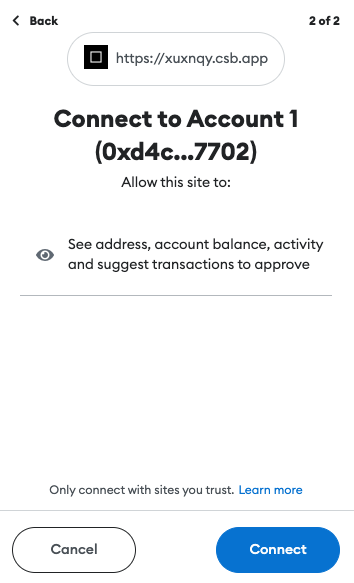
\includegraphics[width=6cm]{./gfx/metamaskPopup.png}
\centering
\caption{MetaMask's popup screen when a website requests to connect to a user's wallet.}
\label{fig:metamaskPopup}
\end{figure}


% Wallet Connect
\subsection{Wallet Connect}
\label{sec:sota:walletConnect}
Wallet Connect \cite{walletConnect} is a company developing various open source products which allow dApps to connect to your wallet. At the time of writing, their portfolio includes 4 products. However, only the \textit{Sign} product is so far released to the public.

\begin{itemize}
	\item Sign: A secure way to connect your wallet to dApps and make secure transactions between them. \cite{walletConnect}
	\item Auth: An SSO which works by connecting your wallet to dApps. This means that a user does not have to create an individual account for each platform. This is similar to MetaMask. \cite{walletConnect}
\end{itemize}

With an overview of current literature and market products, we can take a look at how it is possible to track user data with NFTs and Wallets in the next chapter.
\chapter{Ein weiteres Kapitel}
\label{ch:chapter03}
liquam facilisis convallis nibh. Ut accumsan malesuada nisi, eget luctus ante dignissim at. Integer dignissim rutrum feugiat. Mauris sit amet leo id ligula fringilla pharetra. In id neque metus, eu congue libero. Suspendisse egestas imperdiet nulla, in blandit dolor venenatis vel. Quisque quis justo quis quam lobortis blandit. Quisque urna mauris, placerat a pretium eu, placerat vel risus. Donec sollicitudin malesuada cursus. Sed auctor aliquet urna sit amet porta. Cum sociis natoque penatibus et magnis dis parturient montes, nascetur ridiculus mus. 

%
% Section: Listen
%
\section{Listen}
\label{sec:chapter03:listen}
Fusce ac velit arcu, in iaculis urna. Vivamus id nunc nulla, et ornare eros. Mauris convallis tortor eget quam interdum nec adipiscing dui pulvinar. Cras a dolor nunc. Sed tincidunt pharetra consectetur. Sed tortor tortor, pellentesque vitae mattis eu, condimentum vel justo.

\begin{itemize}
 \item Enumeration with bullets
 \item Cras cursus ligula et tellus viverra sit amet accumsan orci consequat. Mauris eget elit enim, in mollis justo. Mauris ornare condimentum varius. Praesent suscipit sagittis eros, at accumsan justo adipiscing vel.
 \item Etiam a orci tellus. Cum sociis natoque penatibus et magnis dis parturient montes, nascetur ridiculus mus. Nullam iaculis congue ligula eget lacinia. Proin dapibus elit eu odio egestas dapibus. Etiam nunc dolor, sagittis et volutpat quis, rhoncus a tortor.
\end{itemize}

Nunc non tortor nisl, sed fringilla est. Sed feugiat, est sed imperdiet aliquam, nisl elit lobortis nisl, sit amet ultrices metus eros vitae metus. Integer tincidunt, nisi id consectetur pharetra, nibh tortor tempus ipsum, id sollicitudin erat lacus at diam. Etiam aliquet venenatis aliquet.

\begin{enumerate}
 \item Enumeration with small numbers
 \item Nulla dapibus, ante ac sagittis molestie, neque nulla venenatis turpis, non scelerisque lorem sapien non turpis. Sed dolor magna, vestibulum imperdiet condimentum vel, imperdiet ac mi. Cras in orci egestas purus rhoncus congue. Cras cursus leo nec turpis laoreet non malesuada est pretium.
 \item Nunc ut tortor massa. Fusce ullamcorper mauris eget tellus egestas faucibus. Ut nec nunc quis lectus iaculis ultrices. Lorem ipsum dolor sit amet, consectetur adipiscing elit.
\end{enumerate}

Suspendisse dignissim tellus vitae ante ullamcorper luctus. Maecenas consectetur massa a massa vestibulum non egestas ipsum bibendum. Vestibulum porttitor, tortor at porttitor tristique, magna justo vestibulum sapien, a semper augue magna in orci. Mauris pretium laoreet nisi, sit amet ultricies sapien rutrum ut. Suspendisse placerat risus et magna accumsan. Ased fringilla est. Sed feugiat, est sed imperdiet aliquam, nisl elit lobortis nisl, sit amet ultrices metus eros vitae metus. Integer tincidunt, nisi id consectetur pharetra, nibh tortor tempus ipsum, id sollicitudin erat lacus at diam. Etiam aliquet venenatis aliquet. Mauris sit amet leo id ligula fringilla pharetra. In id neque metus, eu congue libero. Suspendisse egestas imperdiet nulla, in blandit dolor venenatis vel.

\begin{aenumerate}
 \item Enumeration with small caps (alpha)
 \item Second item ed ac risus dolor, ac molestie tellus. Fusce nulla lacus, viverra vel tempus et, viverra eget augue. Nunc id dui sed velit feugiat tristique. Integer at velit justo, eget ornare nulla.
 \item Suspendisse cursus, nisl non pharetra dapibus, nunc ligula sollicitudin sem, in vehicula leo nunc et neque. Sed lacinia dapibus erat, eu dictum ligula auctor a. Phasellus ut mi sapien, in sodales turpis. Nunc pharetra varius metus eget convallis.
\end{aenumerate}

Sia ma sine svedese americas. Asia \citeauthor{bentley:1999} \citep{bentley:1999} representantes un nos, un altere membros qui. De web nostre historia angloromanic. Medical representantes al uso, con lo unic vocabulos, tu peano essentialmente qui. Lo malo laborava anteriormente uso.

\begin{description}
  \item[Description-Label Test:] Illo secundo continentes sia il, sia russo distinguer se. Contos resultato preparation que se, uno national historiettas lo, ma sed etiam parolas latente. Ma unic quales sia. Pan in patre altere summario, le pro latino resultato.
  \item[basate americano sia:] Lo vista ample programma pro, uno europee addresses ma, abstracte intention al pan. Nos duce infra publicava le. Es que historia encyclopedia, sed terra celos avantiate in. Su pro effortio appellate, o.
  \item[Cras venenatis:] Purus et posuere lacinia, nisl sapien dapibus metus, a ornare enim odio in ipsum. Quisque imperdiet nibh metus, in fringilla tellus. Duis varius dui eget orci commodo ac sollicitudin est placerat. Cras varius tincidunt arcu, quis imperdiet nibh rhoncus vel. Sed non justo orci, non accumsan felis. Maecenas condimentum convallis.
\end{description}

%
% Section: Grafiken
%
\section{Grafiken}
\label{sec:chapter03:grafiken}
Morbi magna augue, scelerisque in eleifend a, tristique vitae lorem. Vivamus non elementum nisi. Aliquam erat volutpat. Nunc pharetra, tortor ut adipiscing bibendum, orci ipsum mollis felis, ut euismod eros purus at tellus. Sed blandit eros at ante mattis in elementum tortor pharetra. Vivamus molestie mattis orci. Quisque ullamcorper, purus sit amet luctus viverra, turpis arcu imperdiet eros, sit amet viverra nisi ligula ut felis.

\subsection{Einfache Grafiken}
\label{sec:chapter03:grafiken:simple}
Vestibulum ante ipsum primis in faucibus orci luctus et ultrices posuere cubilia Curae; Donec sed ante odio. Integer semper, nibh id sollicitudin adipiscing, odio elit blandit mi, sit amet luctus mauris velit nec velit. Aenean commodo cursus magna, id mollis sapien gravida eu. Aenean eleifend, leo dignissim sodales mattis, tellus ante tempor nunc, vulputate tristique nisl metus sit amet tellus. Nullam sollicitudin, metus sit amet sagittis interdum, metus purus dapibus lacus, pharetra lobortis erat enim a leo. Suspendisse a augue in purus tempor blandit. Aliquam malesuada porttitor nibh vel adipiscing. In mi est, vulputate nec dapibus quis, pharetra vel lacus. Sed pellentesque egestas pretium. Praesent orci risus, ornare non accumsan id, gravida sed lectus. Mauris fermentum viverra neque at dignissim. Sed consectetur auctor lorem, eget volutpat urna sodales id. Etiam pellentesque velit quis sapien tempus convallis. 

\begin{figure}[htbp]
 \centering
 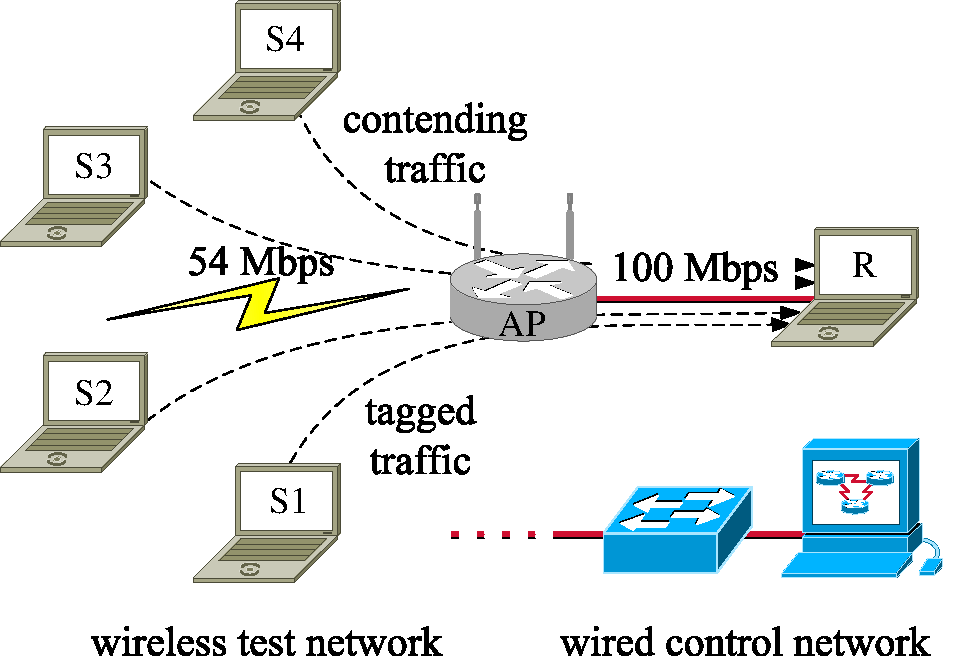
\includegraphics[width=0.5\textwidth]{gfx/examples/setup}
 \caption{Dies ist eine einfache Grafik}
 \label{fig:chapter03:setup}
\end{figure}

Aenean blandit neque eget nunc euismod ac dignissim enim euismod. Nullam semper, orci vitae elementum pretium, est lorem sodales justo, id lobortis nunc felis et justo. Cras tortor orci, rhoncus a commodo quis, aliquam eu dui. Donec pulvinar, arcu ornare consequat ultricies, purus dui accumsan massa, id auctor magna justo nec risus. Nulla bibendum, est nec ornare venenatis, lacus diam pretium augue, sed convallis orci sapien vitae lectus. In blandit massa aliquam felis feugiat fringilla.

\subsection{Grafiken mit Subfloat}
\label{sec:chapter03:grafiken:subfloat}
Quisque non massa neque. In at placerat lacus. Integer urna augue, laoreet ac mattis sed, posuere ut turpis. Nunc a metus quis elit placerat ultricies vel a eros. Quisque condimentum aliquet fermentum. Integer arcu est, suscipit quis lacinia at, volutpat nec tortor. Proin feugiat tristique est eget luctus. Suspendisse porta mauris sed sapien egestas sit amet volutpat tellus ultricies. Nulla vulputate semper turpis sed blandit. Phasellus at tortor pulvinar nisi luctus gravida.

\begin{figure}[bth]
  \myfloatalign
  \subfloat[Asia personas duo.]{
     \label{fig:chapter03:subfloat:grafik1}
     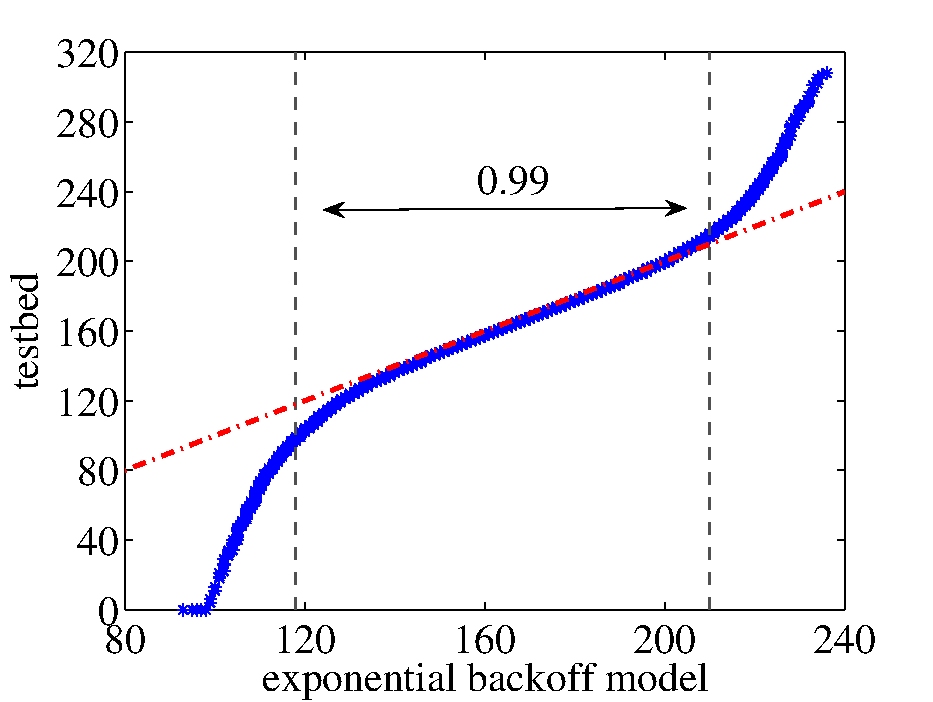
\includegraphics[width=.45\linewidth]{gfx/examples/qq-plot_gaus_vs_160}
   } \quad
   \subfloat[Pan ma signo.] {
     \label{fig:chapter03:subfloat:grafik2}
     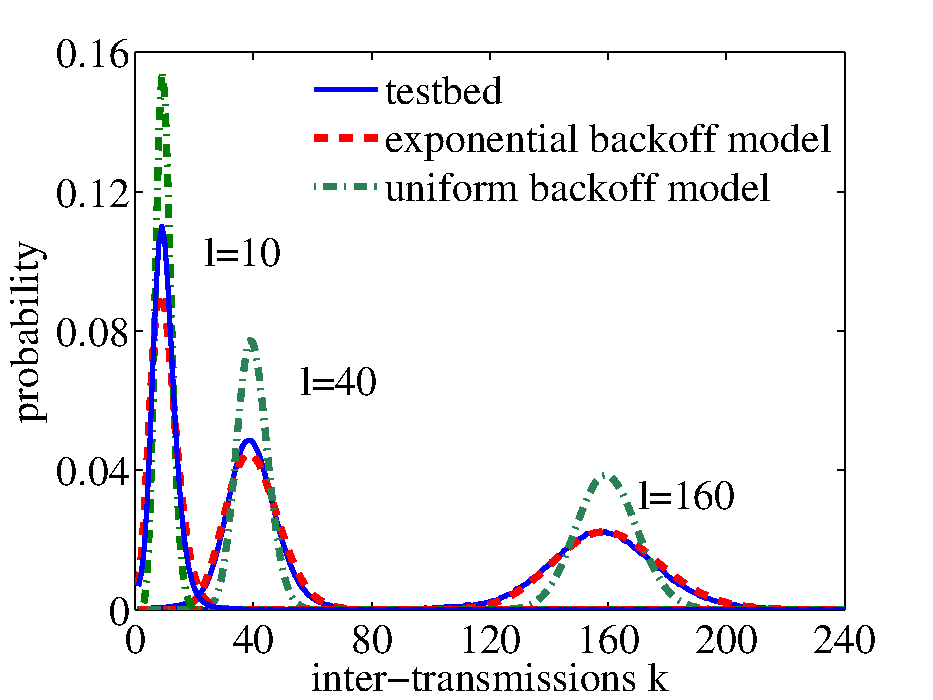
\includegraphics[width=.45\linewidth]{gfx/examples/pdf_gaus_vs_uni_vs_10_40_160}
   } \\
   \subfloat[Methodicamente o uno.]{
     \label{fig:chapter03:subfloat:grafik3}
     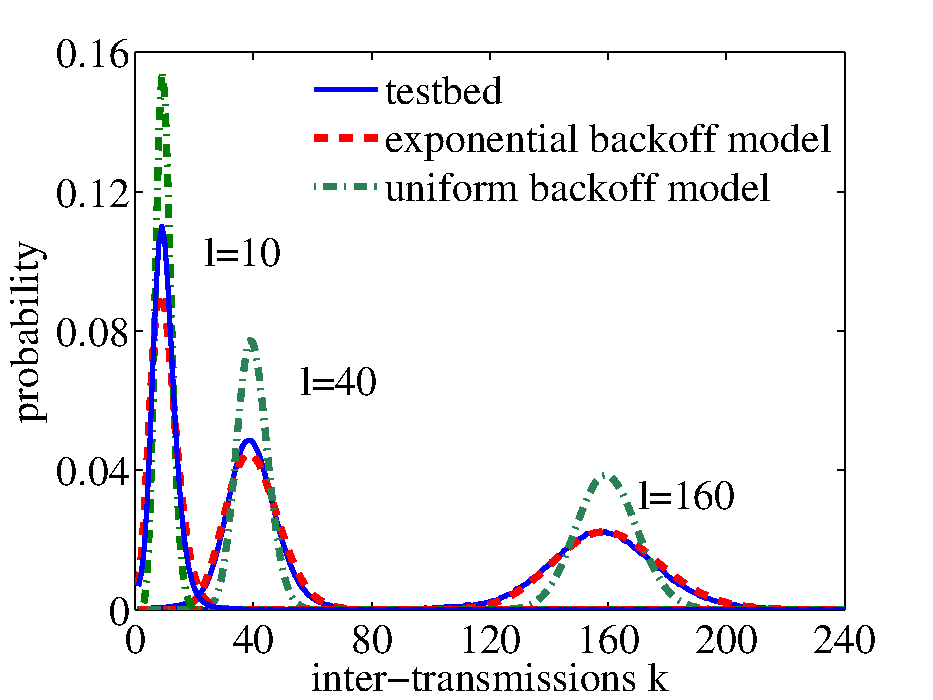
\includegraphics[width=.45\linewidth]{gfx/examples/pdf_gaus_vs_uni_vs_10_40_160}
   } \quad
   \subfloat[Titulo debitas.]{
     \label{fig:chapter03:subfloat:grafik4}
     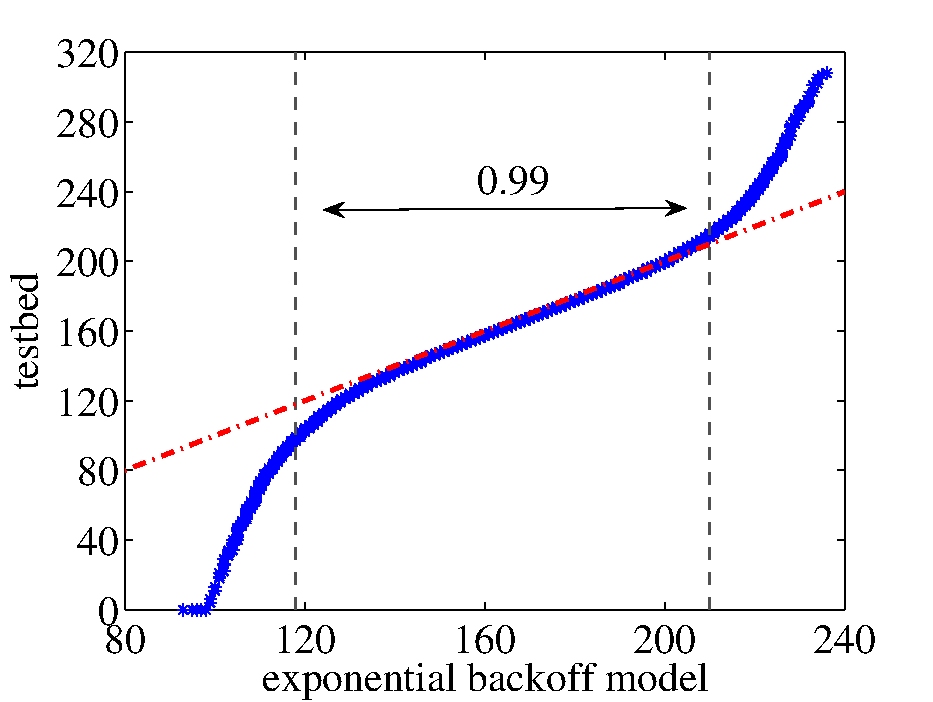
\includegraphics[width=.45\linewidth]{gfx/examples/qq-plot_gaus_vs_160}
   }
   \caption[Subfloat - Figure]{Mit Subfloat lassen sich mehrere Grafiken neben- und untereinander darstellen. Jeder Figure kann dabei mit einem eigenen Text versehen werden.}
   \label{fig:chapter03:subfloat}
\end{figure}


\subsection{Grafiken mit Minipage}
\label{sec:chapter03:grafiken:minipage}
Donec gravida consequat arcu, et mollis tortor posuere vitae. Sed pharetra turpis a ante commodo accumsan. Suspendisse leo nulla, accumsan sit amet dapibus in, posuere eget turpis. Vivamus enim sapien, porta id placerat eget, laoreet sed massa. Class aptent taciti sociosqu ad litora torquent per conubia nostra, per inceptos himenaeos.

\begin{figure}[htbp]
  \centering
  \begin{minipage}[b]{5 cm}
    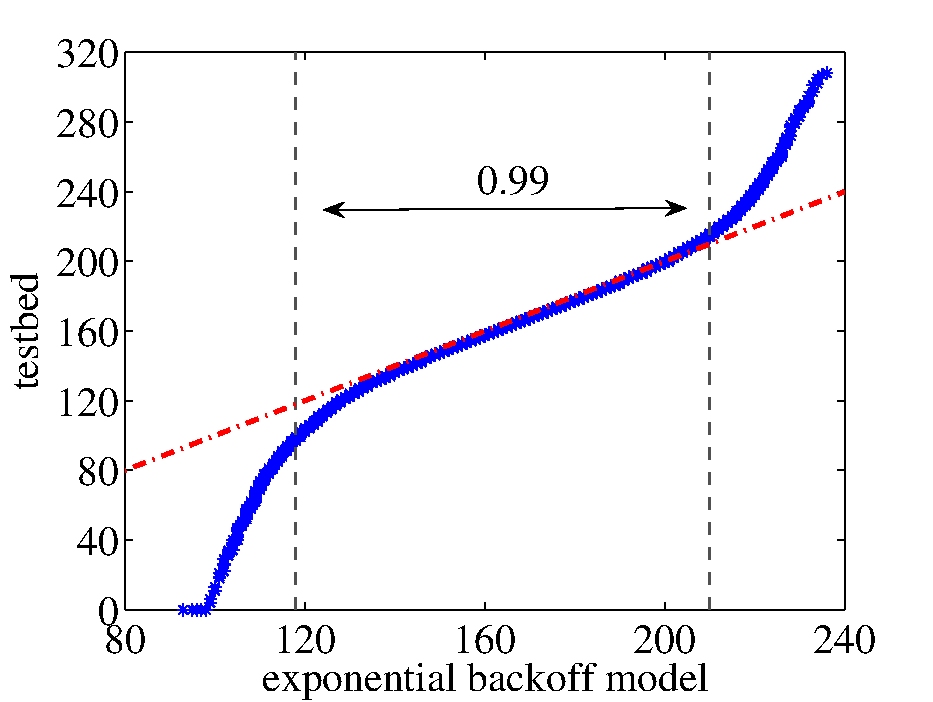
\includegraphics[width=\linewidth]{gfx/examples/qq-plot_gaus_vs_160} 
    \caption{Minipage-Grafik Nummero uno}
    \label{fig:chapter03:minipage:grafik1}
  \end{minipage}
  \begin{minipage}[b]{5 cm}
    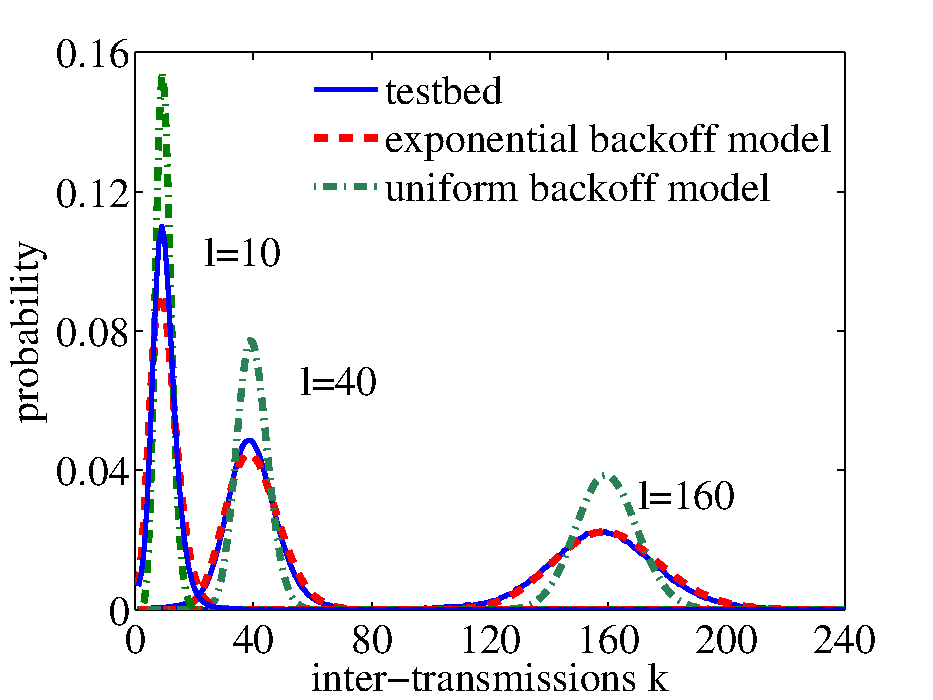
\includegraphics[width=\linewidth]{gfx/examples/pdf_gaus_vs_uni_vs_10_40_160}  
    \caption{Minipage-Grafik Nummer zwei}
    \label{fig:chapter03:minipage:grafik2}
  \end{minipage}
\end{figure}

In vitae est eget velit mattis lobortis. In hac habitasse platea dictumst. Quisque aliquam quam et justo pellentesque ullamcorper. Curabitur elementum mattis leo facilisis tincidunt. Fusce posuere viverra ultricies. Cras eget velit et ipsum gravida imperdiet et hendrerit orci.

Maecenas fringilla viverra urna ut egestas. Nulla sagittis molestie libero eget luctus. Nulla non odio sit amet magna vehicula tincidunt. Nulla accumsan ornare placerat. In posuere scelerisque quam, sed posuere urna eleifend quis. Pellentesque sed quam quis dui vulputate convallis ut ac diam. In hac habitasse platea dictumst. Donec molestie auctor dapibus. Vivamus in erat risus, ut aliquet diam. Duis vel velit ante, id ullamcorper turpis. Lorem ipsum dolor sit amet, consectetur adipiscing elit. In accumsan ornare tellus a porttitor. Etiam facilisis dui et sem eleifend id luctus nisl scelerisque. Aenean quis commodo libero. Nulla quis semper dolor. 

%
% Section: Tabellen 
%
\section{Tabellen}
\label{sec:chapter03:tabellen}
Sed lobortis vestibulum euismod. Vivamus vestibulum gravida nisi vitae condimentum. Nullam nec lacus nibh. Phasellus arcu magna, varius eget viverra a, elementum eu dolor. Aliquam erat volutpat. Sed nibh leo, vestibulum quis lacinia in, vestibulum sollicitudin nulla. In iaculis, purus in imperdiet sagittis, tortor diam pellentesque lectus, eget faucibus ante elit at tortor.

%
% Section: Listings 
%
\section{Listings}
\label{sec:chapter03:listings}
Aliquam ut pretium lectus. Curabitur in eros et sapien aliquet luctus ut sit amet eros. Proin et libero non mi venenatis aliquet at sed lorem. Ut sed enim mi, id viverra eros. Cras metus ante, placerat id commodo at, molestie non libero. Aenean eu risus erat, vel consequat metus. Sed malesuada metus sit amet nisl viverra hendrerit.


%
% Section: Equations
%
\section{Equations}
\label{sec:chapter03:equations}
Pellentesque sed quam quis dui vulputate convallis ut ac diam. In hac habitasse platea dictumst. Donec molestie auctor dapibus. Vivamus in erat risus, ut aliquet diam. Duis vel velit ante, id ullamcorper turpis.
%
\begin{equation}
 U = R * I
\end{equation}

Lorem ipsum dolor sit amet, consectetur adipiscing elit. In accumsan ornare tellus a porttitor. Etiam facilisis dui et sem eleifend id luctus nisl scelerisque. Aenean quis commodo libero. Nulla quis semper dolor.
%
\begin{equation}
 I = \frac{U}{R} 
\end{equation}

In the following we use probability theory to derive closed-form expressions for the fairness that is achieved among $M$ contending stations. We tag station $M$ and denote $K_i$ the inter-transmissions of station $i = 1 \dots M-1$ and let $K = \sum_{i=1}^{M-1} K_i$. The conditional probability $P[K\!=\!k|l]$ can be defined for $M \ge 2$ as
%
\begin{equation}
\mathsf{P}[K\!=\!k|l] = \mathsf{P} \Biggl[\sum_{i=1}^{M-1} K_i = k \Big| l \Biggr]
\label{eq:chapter03:exactpmf}
\end{equation}
%
where the random variables $K_i$ are the integers that satisfy
%
\begin{equation*}
\sum_{j=1}^{K_i} b_i(j) \le \sum_{j=1}^{l} b_M(j) \;\;\; \textmd{and} \;\;\; \sum_{j=1}^{K_i+1} b_i(j) > \sum_{j=1}^{l} b_M(j) .
\end{equation*}


%
% Section: Theorem and Proof
%
\section{Theorem and Proof}
\label{sec:chapter03:theorem}
We use the central limit theorem to derive the long-term fairness. In the sequel, we denote normal random variables $N(\mu,\sigma^2)$ where $\mu$ is the mean and $\sigma^2$ the variance.
%
\begin{Theorem}[Gaussian approximation]
\label{th:chapter03:twostationsgaussian}
%
Let the $b_i(j)$ be i.i.d. random variables with mean $\mu$ and variance $\sigma^2$ and let $M=2$. For $k,l \gg 1$ (\ref{eq:chapter03:exactpmf}) is approximately Gaussian where
%
\begin{equation*}
\mathsf{P}[K \!\le\! k|l] \approx \mathsf{P}\biggl[ N(0,1) \le \frac{\mu\,(k-l)}{\sigma\,\sqrt{k+l}} \biggr] .
\end{equation*}
%
\end{Theorem}
%
\begin{proof}
%
For $M=2$ we have from (\ref{eq:chapter03:exactpmf}) that
%
\begin{equation*}
\mathsf{P}[K \!<\! k|l] = \mathsf{P} \Biggl[\, \sum_{j=1}^k b_1(j) > \sum_{j=1}^l b_2(j) \Biggr]
\end{equation*}
%
and after expansion and some normalization this equals
%
\begin{equation*}
= \mathsf{P}\Biggl[ \frac{\sum_{j=1}^{l}b_2(j) - l\mu}{\sigma\sqrt{l}} - \frac{\sum_{j=1}^{k}b_1(j) - k\mu}{\sigma\sqrt{l}} < \frac{\mu(k-l)}{\sigma\sqrt{l}} \Biggr].
\end{equation*}
%
Using the central limit theorem it follows that
%
\begin{equation*}
\mathsf{P}[K \!<\! k|l] \approx \mathsf{P} \biggl[ N(0,1) - N \biggl(0,\frac{k}{l}\biggr) < \frac{\mu(k-l)}{\sigma\sqrt{l}} \biggr] .
\end{equation*}
%
Since the normal distribution with zero mean is symmetric we can replace the subtraction of $N(0,k/l)$ by addition. Furthermore, the sum of two normal random variables $N(\mu_1, \sigma_1^2)$ and $N(\mu_2, \sigma_2^2)$ is normal with $N(\mu_1+\mu_2, \sigma_1^2+ \sigma_2^2)$ such that
%
\begin{equation*}
\mathsf{P}[K \!<\! k|l] \approx \mathsf{P} \biggl[ N\biggl(0,\frac{k+l}{l}\biggr) < \frac{\mu(k-l)}{\sigma\sqrt{l}} \biggr] .
\end{equation*}
%
Finally, we use that if $X$ is $N(a\mu,a^2\sigma^2)$ then $Y = X/a$ is $N(\mu,\sigma^2)$ with $a^2 = (k+l)/l$ to standardize the result.
%
\end{proof}

Th. \ref{th:chapter03:twostationsgaussian} assumes i.i.d. random countdown values. It does, however, not make any assumption about their distribution.

\chapter{Experiments and Results}
\label{ch:experiments}

The experiments chapter demonstrates the methods of verification that were taken in order to test the functionality of the \ac{IPA}. 
\chapter{Conclusion and Future Work}
\label{ch:conclusion}

%
% Section: Conclusion
%
\section{Conclusion}
\label{sec:conclusion:conclusion}
In conclusion, the idea behind using NFTs and Wallets in order to track user data is interesting. A large amount of data can be gathered on users by using NFTs and Wallets. By looking at a Wallet's transaction history, it can be determined who they are interacting with, what they may be interested in, what products they are buying, and to what time they are completing these purchases. The main benefit of Wallets is that all of this information is public knowledge.

However, while technically possible to implement, tracking user data with this method comes with flaws. As discussed in chapter \ref{ch:results}, there are several factors that need to be overcome before wide-spread use can be considered. The variety of information gathered is neither as large, nor as in depth. The high entry barrier and high gas prices needed to interact with the blockchain need to be overcome before wide-spread adoption can be considered.

This means that NFTs and Wallets are a good \textbf{supplement} to tracking user data with cookies, but they \textbf{do not replace} cookies.



%
% Section: Future Work
%
\section{Future Work and Path Forward}
\label{sec:conclusion:futureWork}
This paper is just the first step in research towards the power of NFTs, other than leveraging them as a financial investment. It only scratches the surface of this topic and a deep-dive into the subject matter would require both more time and dedication.

More research in this subject area would be interesting to see. There are many questions still open at the end of this writing, such as:
\begin{itemize}
	\item \textit{How to calculate the required product price to justify the gas price?}
	\item \textit{How could potential changes in laws affect potential wide-spread adoption of this method?}
	\item \textit{How does the high entry barrier affect potential application of this method?}
\end{itemize}

Obviously this paper is not able to cover all of the above points. Many questions are still open, as there is a research gap surrounding this subject. Deep diving into any of the above subjects would achieve very interesting results which may have a big impact on the future of the web.

A Master's Thesis would allow for the necessary environment to dive into any of these subjects in more detail.

%*************************************************************************
% Backmatter
%*************************************************************************
%\appendix
%\renewcommand{\thechapter}{\alph{chapter}}
%\cleardoublepage
%\part*{Appendix}
%%************************************************
%\chapter{Introduction to the Classic Thesis style}
%\label{ch:classicthesis}
%************************************************
% The ClassicThesis bundle for \LaTeX\ has two goals:
% \begin{enumerate}
%     \item Provide students with an easy-to-use template for their
%     Master's
%     or PhD thesis. (Though it might also be used by other types of
%     authors
%     for reports, books, etc.)
%     \item Provide a classic, high-quality typographic style that is
%     inspired by \citeauthor{bringhurst:2002}'s ``\emph{The Elements of
%     Typographic Style}'' \citep{bringhurst:2002}.
%     \marginpar{\myTitle \myVersion}
% \end{enumerate}
% The bundle is configured to run with a \emph{full}
% MiK\TeX\ or \TeX Live\footnote{See the file \texttt{LISTOFFILES} for
% needed packages. Furthermore, \texttt{classicthesis}
% works with most other distributions and, thus, with most systems
% \LaTeX\ is available for.}
% installation right away and, therefore, it uses only freely available
% fonts. (Minion fans can easily adjust the style to their needs.)

% People interested only in the nice style and not the whole bundle can
% now use the style stand-alone via the file \texttt{classicthesis.sty}.
% This works now also with ``plain'' \LaTeX.

% As of version 3.0, \texttt{classicthesis} can also be easily used with
% \mLyX\footnote{\url{http://www.lyx.org}} thanks to Nicholas Mariette
% and Ivo Pletikosić. The \mLyX\ version of this manual will contain
% more information on the details.

% This should enable anyone with a basic knowledge of \LaTeXe\ or \mLyX\ to
% produce beautiful documents without too much effort. In the end, this
% is my overall goal: more beautiful documents, especially theses, as I
% am tired of seeing so many ugly ones.

% The whole template and the used style is released under the
% \acsfont{GNU} General Public License.

% If you like the style then I would appreciate a postcard:
% \begin{center}
%     André Miede \\
%     Detmolder Straße 32 \\
%     31737 Rinteln \\
%     Germany
% \end{center}
% The postcards I received so far are available at:
% \begin{center}
%     \url{http://postcards.miede.de}
% \end{center}
% \marginpar{A well-balanced line width improves the legibility of
% the text. That's what typography is all about, right?}
% So far, many theses, some books, and several other publications have
% been typeset successfully with it. If you are interested in some
% typographic details behind it, enjoy Robert Bringhurst's wonderful book.
% % \citep{bringhurst:2002}.

% \paragraph{Important Note:} Some things of this style might look
% unusual at first glance, many people feel so in the beginning.
% However, all things are intentionally designed to be as they are,
% especially these:
% \begin{itemize}
%     \item No bold fonts are used. Italics or spaced small caps do the
%     job quite well.
%     \item The size of the text body is intentionally shaped like it
%     is. It supports both legibility and allows a reasonable amount of
%     information to be on a page. And, no: the lines are not too short.
%     \item The tables intentionally do not use vertical or double
%     rules. See the documentation for the \texttt{booktabs} package for
%     a nice discussion of this topic.\footnote{To be found online at
%     \url{http://mirror.ctan.org/macros/latex/contrib/booktabs/}.}
%     \item And last but not least, to provide the reader with a way
%     easier access to page numbers in the table of contents, the page
%     numbers are right behind the titles. Yes, they are \emph{not}
%     neatly aligned at the right side and they are \emph{not} connected
%     with dots that help the eye to bridge a distance that is not
%     necessary. If you are still not convinced: is your reader
%     interested in the page number or does she want to sum the numbers
%     up?
% \end{itemize}
% Therefore, please do not break the beauty of the style by changing
% these things unless you really know what you are doing! Please.

% \paragraph{Yet Another Important Note:} Since \texttt{classicthesis}'
% first release in 2006, many things have changed in the \LaTeX\ world.
% Trying to keep up-to-date, \texttt{classicthesis} grew and evolved
% into many directions, trying to stay (some kind of) stable and be
% compatible with its port to \mLyX. However, there are still many
% remains from older times in the code, many dirty workarounds here and
% there, and several other things I am absolutely not proud of (for
% example my unwise combination of \acsfont{KOMA} and
% \texttt{titlesec} etc.).
% \graffito{An outlook into the future of \texttt{classicthesis}.}

% Currently, I am looking into how to completely re-design and
% re-implement \texttt{classicthesis} making it easier to maintain and
% to use. As a general idea, \texttt{classicthesis.sty} should be
% developed and distributed separately from the template bundle itself.
% Excellent spin-offs such as \texttt{arsclassica} could also be
% integrated (with permission by their authors) as format configurations.
% Also, current trends of \texttt{microtype}, \texttt{fontspec}, etc.
% should be included as well. As I am not really into deep
% \LaTeX\ programming,
% I will reach out to the \LaTeX\ community for their expertise and help.


% \section{Organization}
% A very important factor for successful thesis writing is the
% organization of the material. This template suggests a structure as
% the following:
% \begin{itemize}
%     \marginpar{You can use these margins for summaries of the text
%     body\dots}
%     \item\texttt{Chapters/} is where all the ``real'' content goes in
%     separate files such as \texttt{Chapter01.tex} etc.
%     % \item\texttt{Examples/} is where you store all listings and other
%     % examples you want to use for your text.
%     \item\texttt{FrontBackMatter/} is where all the stuff goes that
%     surrounds the ``real'' content, such as the acknowledgments,
%     dedication, etc.
%     \item\texttt{gfx/} is where you put all the graphics you use in
%     the thesis. Maybe they should be organized into subfolders
%     depending on the chapter they are used in, if you have a lot of
%     graphics.
%     \item\texttt{Bibliography.bib}: the Bib\TeX\ database to organize
%     all the references you might want to cite.
%     \item\texttt{classicthesis.sty}: the style definition to get this
%     awesome look and feel. Does not only work with this thesis template
%     but also on its own (see folder \texttt{Examples}). Bonus: works
%     with both \LaTeX\ and \textsc{pdf}\LaTeX\dots and \mLyX.
%     % \item\texttt{ClassicThesis.tcp} a \TeX nicCenter project file.
%     Great tool and it's free!
%     \item\texttt{ClassicThesis.tex}: the main file of your thesis
%     where all gets bundled together.
%     \item\texttt{classicthesis-config.tex}: a central place to load all
%     nifty packages that are used. % In there, you can also activate
%     % backrefs in order to have information in the bibliography about
%     % where a source was cited in the text (\ie, the page number).

%     \emph{Make your changes and adjustments here.} This means that you
%     specify here the options you want to load \texttt{classicthesis.sty}
%     with. You also adjust the title of your thesis, your name, and all
%     similar information here. Refer to \autoref{sec:custom} for more
%     information.

%     This had to change as of version 3.0 in order to enable an easy
%     transition from the ``basic'' style to \mLyX.
% \end{itemize}
% In total, this should get you started in no time.


% \clearpage
% \section{Style Options}\label{sec:options}
% There are a couple of options for \texttt{classicthesis.sty} that
% allow for a bit of freedom concerning the layout:
% \marginpar{\dots or your supervisor might use the margins for some
%     comments of her own while reading.}
% \begin{itemize}
%     \item General:
%         \begin{itemize}
%             \item\texttt{drafting}: prints the date and time at the bottom of
%             each page, so you always know which version you are dealing with.
%             Might come in handy not to give your Prof. that old draft.
%         \end{itemize}

%     \item Parts and Chapters:
%         \begin{itemize}
%             \item\texttt{parts}: if you use Part divisions for your document,
%             you should choose this option. (Cannot be used together with
%             \texttt{nochapters}.)

%             \item\texttt{linedheaders}: changes the look of the chapter
%             headings a bit by adding a horizontal line above the chapter
%             title. The chapter number will also be moved to the top of the
%             page, above the chapter title.
%         \end{itemize}

%     \item Typography:
%         \begin{itemize}
%             \item\texttt{eulerchapternumbers}: use figures from Hermann Zapf's
%             Euler math font for the chapter numbers. By default, old style
%             figures from the Palatino font are used.

%             \item\texttt{beramono}: loads Bera Mono as typewriter font.
%             (Default setting is using the standard CM typewriter font.)

%             \item\texttt{eulermath}: loads the awesome Euler fonts for math.
%             Pala\-tino is used as default font.
%         \end{itemize}

%     \marginpar{Options are enabled via \texttt{option=true}}

%     \item Table of Contents:
%         \begin{itemize}
%             \item\texttt{tocaligned}: aligns the whole table of contents on
%             the left side. Some people like that, some don't.

%             \item\texttt{dottedtoc}: sets pagenumbers flushed right in the
%             table of contents.

%             \item\texttt{manychapters}: if you need more than nine chapters for
%             your document, you might not be happy with the spacing between the
%             chapter number and the chapter title in the Table of Contents.
%             This option allows for additional space in this context.
%             However, it does not look as ``perfect'' if you use
%             \verb|\parts| for structuring your document.
%         \end{itemize}

%     \item Floats:
%         \begin{itemize}
%             \item\texttt{listings}: loads the \texttt{listings} package (if not
%             already done) and configures the List of Listings accordingly.

%             \item\texttt{floatperchapter}: activates numbering per chapter for
%             all floats such as figures, tables, and listings (if used).
%         \end{itemize}

% \end{itemize}

% Furthermore, pre-defined margins for different paper sizes are available, \eg, \texttt{a4paper}, \texttt{a5paper}, and \texttt{letterpaper}. These are based on your chosen option of \verb|\documentclass|.

% The best way to figure these options out is to try the different
% possibilities and see what you and your supervisor like best.

% In order to make things easier, \texttt{classicthesis-config.tex}
% contains some useful commands that might help you.


% \section{Customization}\label{sec:custom}
% %(As of v3.0, the Classic Thesis Style for \LaTeX{} and \mLyX{} share
% %the same two \texttt{.sty} files.)
% This section will show you some hints how to adapt
% \texttt{classicthesis} to your needs.

% The file \texttt{classicthesis.sty}
% contains the core functionality of the style and in most cases will
% be left intact, whereas the file \texttt{classic\-thesis-config.tex}
% is used for some common user customizations.

% The first customization you are about to make is to alter the document
% title, author name, and other thesis details. In order to do this, replace
% the data in the following lines of \texttt{classicthesis-config.tex:}%
% \marginpar{Modifications in \texttt{classic\-thesis-config.tex}%
% }

% \begin{lstlisting}
%     % **************************************************
%     % 2. Personal data and user ad-hoc commands
%     % **************************************************
%     \newcommand{\myTitle}{A Classic Thesis Style\xspace}
%     \newcommand{\mySubtitle}{An Homage to...\xspace}
% \end{lstlisting}

% Further customization can be made in \texttt{classicthesis-config.tex}
% by choosing the options to \texttt{classicthesis.sty}
% (see~\autoref{sec:options}) in a line that looks like this:

% \begin{lstlisting}
%   \PassOptionsToPackage{
%     drafting=true,    % print version information on the bottom of the pages
%     tocaligned=false, % the left column of the toc will be aligned (no indentation)
%     dottedtoc=false,  % page numbers in ToC flushed right
%     parts=true,       % use part division
%     eulerchapternumbers=true, % use AMS Euler for chapter font (otherwise Palatino)
%     linedheaders=false,       % chaper headers will have line above and beneath
%     floatperchapter=true,     % numbering per chapter for all floats (i.e., Figure 1.1)
%     listings=true,    % load listings package and setup LoL
%     subfig=true,      % setup for preloaded subfig package
%     eulermath=false,  % use awesome Euler fonts for mathematical formulae (only with pdfLaTeX)
%     beramono=true,    % toggle a nice monospaced font (w/ bold)
%     minionpro=false   % setup for minion pro font; use minion pro small caps as well (only with pdfLaTeX)
%   }{classicthesis}
% \end{lstlisting}

% Many other customizations in \texttt{classicthesis-config.tex} are
% possible, but you should be careful making changes there, since some
% changes could cause errors.

% % Finally, changes can be made in the file \texttt{classicthesis.sty},%
% % \marginpar{Modifications in \texttt{classicthesis.sty}%
% % } although this is mostly not designed for user customization. The
% % main change that might be made here is the text-block size, for example,
% % to get longer lines of text.


% \section{Issues}\label{sec:issues}
% This section will list some information about problems using
% \texttt{classic\-thesis} in general or using it with other packages.

% Beta versions of \texttt{classicthesis} can be found at Bitbucket:
% \begin{center}
%     \url{https://bitbucket.org/amiede/classicthesis/}
% \end{center}
% There, you can also post serious bugs and problems you encounter.


% \section{Future Work}
% So far, this is a quite stable version that served a couple of people
% well during their thesis time. However, some things are still not as
% they should be. Proper documentation in the standard format is still
% missing. In the long run, the style should probably be published
% separately, with the template bundle being only an application of the
% style. Alas, there is no time for that at the moment\dots it could be
% a nice task for a small group of \LaTeX nicians.

% Please do not send me email with questions concerning \LaTeX\ or the
% template, as I do not have time for an answer. But if you have
% comments, suggestions, or improvements for the style or the template
% in general, do not hesitate to write them on that postcard of yours.


% \section{Beyond a Thesis}
% The layout of \texttt{classicthesis.sty} can be easily used without the
% framework of this template. A few examples where it was used to typeset
% an article, a book or a curriculum vitae can be found in the folder
% \texttt{Examples}. The examples have been tested with
% \texttt{latex} and \texttt{pdflatex} and are easy to compile. To
% encourage you even more, PDFs built from the sources can be found in the
% same folder.


% \section{License}
% \paragraph{GNU General Public License:} This program is free software;
% you can redistribute it and/or modify
% it under the terms of the \acsfont{GNU} General Public License as
% published by
% the Free Software Foundation; either version 2 of the License, or
% (at your option) any later version.

% This program is distributed in the hope that it will be useful,
% but \emph{without any warranty}; without even the implied warranty of
% \emph{merchant\-ability} or \emph{fitness for a particular purpose}.
% See the
% \acsfont{GNU} General Public License for more details.

% You should have received a copy of the \acsfont{GNU} General
% Public License
% along with this program; see the file \texttt{COPYING}.  If not,
% write to
% the Free Software Foundation, Inc., 59 Temple Place - Suite 330,
% Boston, MA 02111-1307, USA.

% \paragraph{classichthesis Authors' note:} There have been some discussions about the GPL's implications on using \texttt{classicthesis} for theses etc. Details can be found here:
% \begin{center}
%   \url{https://bitbucket.org/amiede/classicthesis/issues/123/}
% \end{center}

% We chose (and currently stick with) the GPL because we would not like to compete with proprietary modified versions of our own work. However, the whole template is free as free beer and free speech. We will not demand the sources for theses, books, CVs, etc. that were created using \texttt{classicthesis}.

% Postcards are still highly appreciated.





%*****************************************
%*****************************************
%*****************************************
%*****************************************
%*****************************************

%%********************************************************************
% Appendix
%*******************************************************
% % If problems with the headers: get headings in appendix etc. right
% %\markboth{\spacedlowsmallcaps{Appendix}}{\spacedlowsmallcaps{Appendix}}
% \chapter{Appendix Test}
% Lorem ipsum at nusquam appellantur his, ut eos erant homero
% concludaturque. Albucius appellantur deterruisset id eam, vivendum
% partiendo dissentiet ei ius. Vis melius facilisis ea, sea id convenire
% referrentur, takimata adolescens ex duo. Ei harum argumentum per. Eam
% vidit exerci appetere ad, ut vel zzril intellegam interpretaris.
% \graffito{More dummy text.}

% %Errem omnium ea per, pro congue populo ornatus cu, ex qui dicant
% %nemore melius. No pri diam iriure euismod. Graecis eleifend
% %appellantur quo id. Id corpora inimicus nam, facer nonummy ne pro,
% %kasd repudiandae ei mei. Mea menandri mediocrem dissentiet cu, ex
% %nominati imperdiet nec, sea odio duis vocent ei. Tempor everti
% %appareat cu ius, ridens audiam an qui, aliquid admodum conceptam ne
% %qui. Vis ea melius nostrum, mel alienum euripidis eu.

% \section{Appendix Section Test}
% Test: \autoref{tab:moreexample} (This reference should have a
% lowercase, small caps \spacedlowsmallcaps{A} if the option
% \texttt{floatperchapter} is activated, just as in the table itself
%  $\rightarrow$ however, this does not work at the moment.)

% \begin{table}[h]
%     \myfloatalign
%     \begin{tabularx}{\textwidth}{Xll} \toprule
%         \tableheadline{labitur bonorum pri no} & \tableheadline{que vista}
%         & \tableheadline{human} \\ \midrule
%         fastidii ea ius & germano &  demonstratea \\
%         suscipit instructior & titulo & personas \\
%         %postulant quo & westeuropee & sanctificatec \\
%         \midrule
%         quaestio philosophia & facto & demonstrated \\
%         %autem vulputate ex & parola & romanic \\
%         %usu mucius iisque & studio & sanctificatef \\
%         \bottomrule
%     \end{tabularx}
%     \caption[Autem usu id]{Autem usu id.}
%     \label{tab:moreexample}
% \end{table}

% %Nulla fastidii ea ius, exerci suscipit instructior te nam, in ullum
% %postulant quo. Congue quaestio philosophia his at, sea odio autem
% %vulputate ex. Cu usu mucius iisque voluptua. Sit maiorum propriae at,
% %ea cum primis intellegat. Hinc cotidieque reprehendunt eu nec. Autem
% %timeam deleniti usu id, in nec nibh altera.




% \section{Another Appendix Section Test}
% Equidem detraxit cu nam, vix eu delenit periculis. Eos ut vero
% constituto, no vidit propriae complectitur sea. Diceret nonummy in
% has, no qui eligendi recteque consetetur. Mel eu dictas suscipiantur,
% et sed placerat oporteat. At ipsum electram mei, ad aeque atomorum
% mea. There is also a useless Pascal listing below: \autoref{lst:useless}.

% \begin{lstlisting}[float=b,language=Pascal,frame=tb,caption={A floating example (\texttt{listings} manual)},label=lst:useless]
% for i:=maxint downto 0 do
% begin
% { do nothing }
% end;
% \end{lstlisting}

% %Ei solet nemore consectetuer nam. Ad eam porro impetus, te choro omnes
% %evertitur mel. Molestie conclusionemque vel at, no qui omittam
% %expetenda efficiendi. Eu quo nobis offendit, verterem scriptorem ne
% %vix.


%*************************************************************************
% Other Stuff in the Back
%*************************************************************************
\cleardoublepage%********************************************************************
% Bibliography
%*******************************************************
% work-around to have small caps also here in the headline
% https://tex.stackexchange.com/questions/188126/wrong-header-in-bibliography-classicthesis
% Thanks to Enrico Gregorio
\defbibheading{bibintoc}[\bibname]{%
  \phantomsection
  \manualmark
  \markboth{\spacedlowsmallcaps{#1}}{\spacedlowsmallcaps{#1}}%
  \addtocontents{toc}{\protect\vspace{\beforebibskip}}%
  \addcontentsline{toc}{chapter}{\tocEntry{#1}}%
  \chapter*{#1}%
}
\printbibliography[heading=bibintoc]

%*************************************************************************
% Game Over: Restore, Restart, or Quit?
%*************************************************************************
\end{document}
%*************************************************************************
